\documentclass[14pt,a4paper]{extarticle}
\usepackage[margin=2cm]{geometry}
\usepackage{graphicx}\graphicspath{{figure/}}\usepackage{float} 
\usepackage[backend=biber]{biblatex}
\usepackage{subcaption} 
\usepackage{mathtools} \usepackage{amsmath}
\usepackage{xcolor}\usepackage{tcolorbox}
\usepackage{listings}\usepackage{adjustbox}
\tcbuselibrary{listingsutf8,skins,fitting}

\newtcolorbox{nota}[0]{
	beforeafter skip balanced=5mm,
	fontupper=\small
}

\definecolor{codegreen}{rgb}{0,0.6,0}
\definecolor{codegray}{rgb}{0.5,0.5,0.5}
\definecolor{codepurple}{rgb}{0.58,0,0.82}
\definecolor{backcolour}{rgb}{0.95,0.95,0.92}
\definecolor{lightgray}{rgb}{0.95,0.95,0.95}

\lstset{
    commentstyle=\color{codegreen},
    numberstyle=\tiny\color{codegray},
    keywordstyle=\color{codepurple},  
    numbers=left,
    language=Matlab,
    basicstyle=\small,
    backgroundcolor=\color{lightgray},
    tabsize=3
}


\addbibresource{bibliografia.bib}

\begin{document}
\numberwithin{equation}{section}
\numberwithin{figure}{section}
\numberwithin{lstlisting}{section}

\begin{titlepage}

\begin{center}
\begin{figure}[H]
\centering

\includegraphics{unical2.png}
\end{figure}
%{\huge\textsc{Università della Calabria}}\\
{\Large Dipartimento di Ingegneria Informatica, Modellistica, Elettronica e Sistemistica}
\vspace{10mm}
\rule{\textwidth}{1pt}\\
\vspace*{5cm}
{\Large Tesi di Laurea in Ingegneria Informatica}\\
\vspace*{0.5cm}
{\huge \textbf{Path planning locale per robot mobili basato su switching tra potenziali artificiali}}
\vspace{5cm}
\end{center}

\begin{minipage}[t]{0.5\textwidth}
%% Relatore %%
{\large{Relatore: \\ \bf Prof. Luigi D'Alfonso}}
\end{minipage}
\hfill
\begin{minipage}[t]{0.4\textwidth}\raggedleft
%% Candidato %%
{\large{Candidato: \\ \bf Flavio Maiorana\\ Mat. 182611}}
\end{minipage}

\begin{center}
\rule{\textwidth}{1pt}\\
ANNO ACCADEMICO 2021/2022
\end{center}

\end{titlepage}

\newpage \tableofcontents \newpage %sommario

\begin{abstract}
Il presente lavoro di tesi ha come obiettivo lo sviluppo, in ambiente Matlab, di un modulo software capace di risolvere un problema di path planning per robot mobili. La soluzione implementata si basa principalmente su quanto descritto in \cite{dalfonso}. L'obiettivo é guidare un robot mobile all'interno di un ambiente non noto, cercando di fargli raggiungere un punto prestabilito, senza collisioni con eventuali ostacoli. La tecnica utilizzata é quella dei potenziali artificiali, ma con un meccanismo di switching a stati. Particolare attenzione é stata posta sullo sviluppo di un'architettura software di supporto alla soluzione implementata. È stato adottato il paradigma della programmazione orientata agli oggetti, sfruttando le funzionalità fornite dal linguaggio Matlab, al fine di rendere il software modulare e riutilizzabile per sviluppi futuri.
\end{abstract}

\section{Introduzione}
È innegabile che in questi anni si stia assistendo ad un aumento vertiginoso di sviluppo ed uso della robotica. È importante però evidenziare una distinzione tra due concetti apparentemente simili, ma per certi versi opposti, che caratterizzano due macro-categorie della robotica: automazione e autonomia.\\ 
\textbf{L'automazione} generalmente riguarda quei robot, tipicamente industriali, che operano in ambienti noti a priori ed eseguono in loop un compito predefinito; automatizzare, perciò, vuol dire sostituire l'essere umano in compiti ripetitivi e solitamente privi di eventi inaspettati.\\
\textbf{L'autonomia}, invece, ben più complessa da realizzare, é caratteristica di quei sistemi che hanno un certo grado di inconsapevolezza sul proprio futuro e l'ambiente circostante.  Il robot, quindi, é definito autonomo se é un agente intelligente situato nello spazio fisico, dove un agente intelligente si definisce come un'entità che \textbf{osserva} l'ambiente e prende delle \textbf{azioni} per ottimizzare il raggiungimento del suo \textbf{obiettivo}\cite{murphy}. Nel caso specifico di questo elaborato, l'ambiente del robot mobile autonomo é lo spazio bidimensionale (una superficie), e il suo obiettivo é un punto in questo spazio. Ottimizzare il raggiungimento di questo punto vuol dire arrivarci nel minor tempo possibile, senza collidere con eventuali ostacoli. Quindi, il robot autonomo deve compiere una serie di azioni, non note a priori e definite da un algoritmo di pianificazione che si basa sui dati osservati dai sensori, per spostare la sua traiettoria, al fine di evitare collisioni e raggiungere comunque l'obiettivo.\\
La tipica architettura di navigazione di un robot autonomo é data perciò da quattro moduli (o primitive): 
\begin{description}
\item[Percezione] Prende in input le informazioni derivanti dai sensori, le processa e le restituisce
\item[Localizzazione e Mapping] Con le informazioni sensoriali, il robot costruisce una rappresentazione del proprio intorno basandosi sulla propria posizione e su ciò che osserva. Il risultato finale, dopo aver fatto varie osservazioni di intorni diversi, sarà una mappa dell'ambiente, rispetto alla quale il robot può localizzarsi. 
\begin{nota}
Per scopi esemplificativi, questo modulo verrà tralasciato nell'algoritmo oggetto del presente elaborato: si userà descrivere la posizione del robot con coordinate assolute e non rispetto ad una mappa
\end{nota}
\item[Pianificazione] In base alle informazioni sensoriali e cognitive in possesso, produce in output delle decisioni ad un livello di astrazione ancora alto. Nel caso del motion planning, la direttiva da produrre é il percorso da seguire. Più in generale, il modulo di pianificazione potrebbe generare delle azioni del tipo ``gira a sinistra", oppure ``fermati".
\item[Azione] Prende in input le direttive del modulo di pianificazione e produce dei comandi a basso livello per gli attuatori del robot.
\end{description}

\begin{figure}[H]
\caption{Architettura di navigazione}
\centering
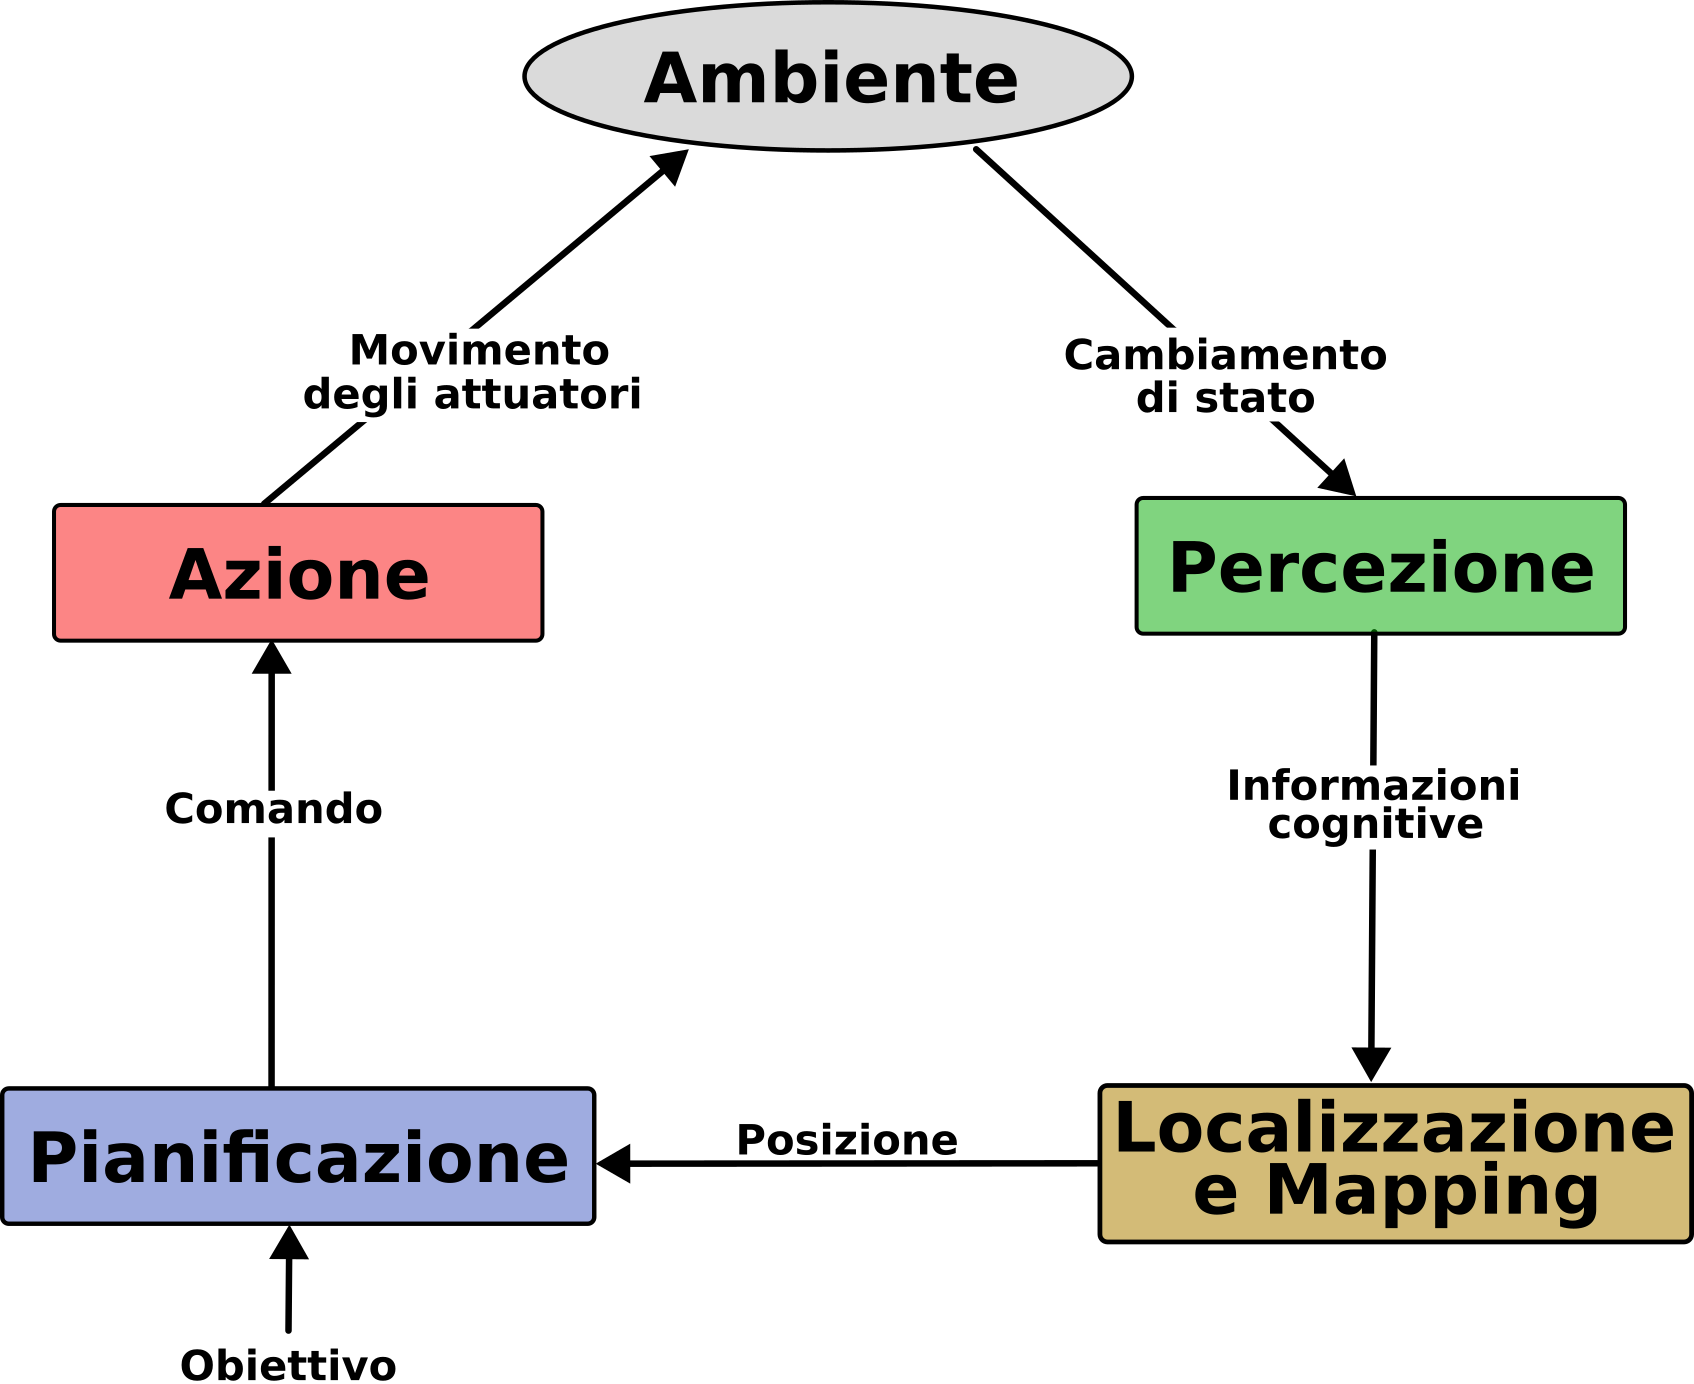
\includegraphics{architecture_tesi.png}
\label{arch}
\end{figure}

L'architettura utilizzata in questa tesi é di tipo gerarchico: le quattro primitive vengono eseguite in ordine e in loop. È particolarmente indicata per problemi in cui l'obiettivo finale é ben definito a priori. In altre parole, non vi é nessun meccanismo di apprendimento nel robot, ma semplicemente pianificazione deterministica orientata al goal. In figura \ref{arch} é visivamente sintetizzato quanto appena detto. Nel presente elaborato viene affrontato un problema che rientra nel terzo modulo: il path planning, un problema di grande importanza e oggetto di interesse nel mondo della ricerca.

\subsection{Path planning}

Una sua rapida formulazione potrebbe essere la seguente: data la posizione iniziale (del robot) A e una posizione finale B, imposta da chi fa uso del robot, il path planning consiste nel calcolare un percorso fisicamente realizzabile e ottimale per arrivare da A a B.\\
Tra i metodi esistenti (e non), ci sono due importanti distinzioni da fare: sulla formulazione del problema e sulla soluzione al problema.
\begin{description}
\item[La prima] é tra online e offline path planning, o anche locale e globale. Il path planning globale riguarda quelle situazioni in cui l'ambiente considerato é interamente noto a priori, per cui é possibile calcolare il percorso da seguire ancor prima che il robot inizi a muoversi; quello locale é inerente ai casi in cui il robot debba fare i conti lungo il suo percorso con eventi inaspettati, ad esempio ostacoli in movimento, caso in cui é necessario reagire localmente, aggiornando ripetutamente le informazioni derivanti dai sensori e aggiustando la traiettoria al fine di evitare l'ostacolo e poter raggiungere in tempi ottimali l'obiettivo. Chiaramente, la quasi totalità dei problemi di robotica autonoma deve fare i conti con una situazione del secondo tipo. 
\item[La seconda] distinzione é tra soluzioni basate su tecniche di intelligenza artificiale - la cui trattazione esula dagli scopi di questa tesi - e soluzioni classiche. Queste ultime possono ulteriormente essere suddivise in \cite{siciliano}:
\begin{itemize}
\item Subgoal (o anche roadmap), la cui realizzazione più nota é il metodo che sfrutta i diagrammi di Voronoi. 
\item Decomposizione in celle
\item Sampling based (sfrutta un approccio probabilistico)
\item Potenziali artificiali, che verranno ampiamente in trattati nel prossimo capitolo
\end{itemize}
\end{description}
Di seguito seguirà una breve descrizione di esempi legati ai metodi appena elencati, con l'intento di motivare la scelta dei potenziali artificiali come base per lo sviluppo dell'algoritmo di navigazione, visto che la totalità dei metodi rientranti nelle prime tre categorie risolve adeguatamente il problema del path planning globale, ma risulta inefficiente nel caso del path planning locale. 
\paragraph{Voronoi} L'idea alla base di questo metodo é rappresentare lo spazio libero delle configurazioni \(C_{free}\) - l'insieme di quei punti che per certo non fanno collidere il robot con un ostacolo - come un grafo, ovvero un insieme di nodi (rappresentanti appunto la roadmap) connessi da archi. La posizione dei nodi é definita tramite il concetto di clearance \[\gamma(q) = \min_{s\in\partial C_{free}} \begin{Vmatrix}q-s\end{Vmatrix}\] dove q é una generica configurazione in \(C_{free}\). La clearence é perciò una funzione che ha come funzione della configurazione \(q\) la distanza minima di \(q\) da un qualunque punto di un ostacolo. Infatti, \(\partial C_{free}\) sarebbe la frontiera dello spazio di configurazione, ovvero il bordo degli ostacoli. \(C_{free}\) é formato da quelle configurazioni \(q\) tali per cui esiste più di un punto sulla frontiera \(\partial C_{free}\) con lo stesso valore \(\gamma(q)\); in altre parole, quei punti equidistanti (considerando la distanza minima) da più di un ostacolo. Il risultato é quello mostrato in figura \ref{voronoi}. Una volta calcolato il grafo, é sufficiente ritrarre i punti di start e goal sul grafo stesso e calcolare il percorso ottimale tra questi due attraverso un algoritmo di ricerca, ad esempio Djikstra.

\paragraph{Decomposizione esatta in celle} In questa tecnica lo spazio delle configurazioni viene suddiviso in celle, come mostrato in figura \ref{celldecomp}. Ogni cella é delimitata inferiormente e superiormente da un ostacolo e ogni cella ha le seguenti due caratteristiche:
\begin{itemize}
\item Tra ogni coppia di configurazioni nella stessa cella esiste sempre un cammino senza collisioni
\item Tra ogni coppia di celle adiacenti esiste sempre un cammino senza collisioni (che conduce da una cella all'altra)
\end{itemize}
In base a questi due principi, viene costruito il cosiddetto grafo di connettività, che ha come archi le connessioni tra celle adiacenti. Come nel metodo precedente, il calcolo del percorso ottimale per raggiungere il goal consiste nell'applicare un algoritmo di ricerca su grafo.

\paragraph{Sampling based} Il terzo metodo si basa su un approccio probabilistico. Brevemente, l'idea é di scegliere a ogni iterazione una configurazione ``di prova" e fare un test di collisione su quest'ultima, cercando poi di costruire un percorso idoneo in base alla vicinanza alle configurazioni già appartenenti al grafo che si sta costruendo. \\

\begin{figure}[H]
\begin{subfigure}[t]{0.5\textwidth}
\centering
\caption{Diagramma di Voronoi}
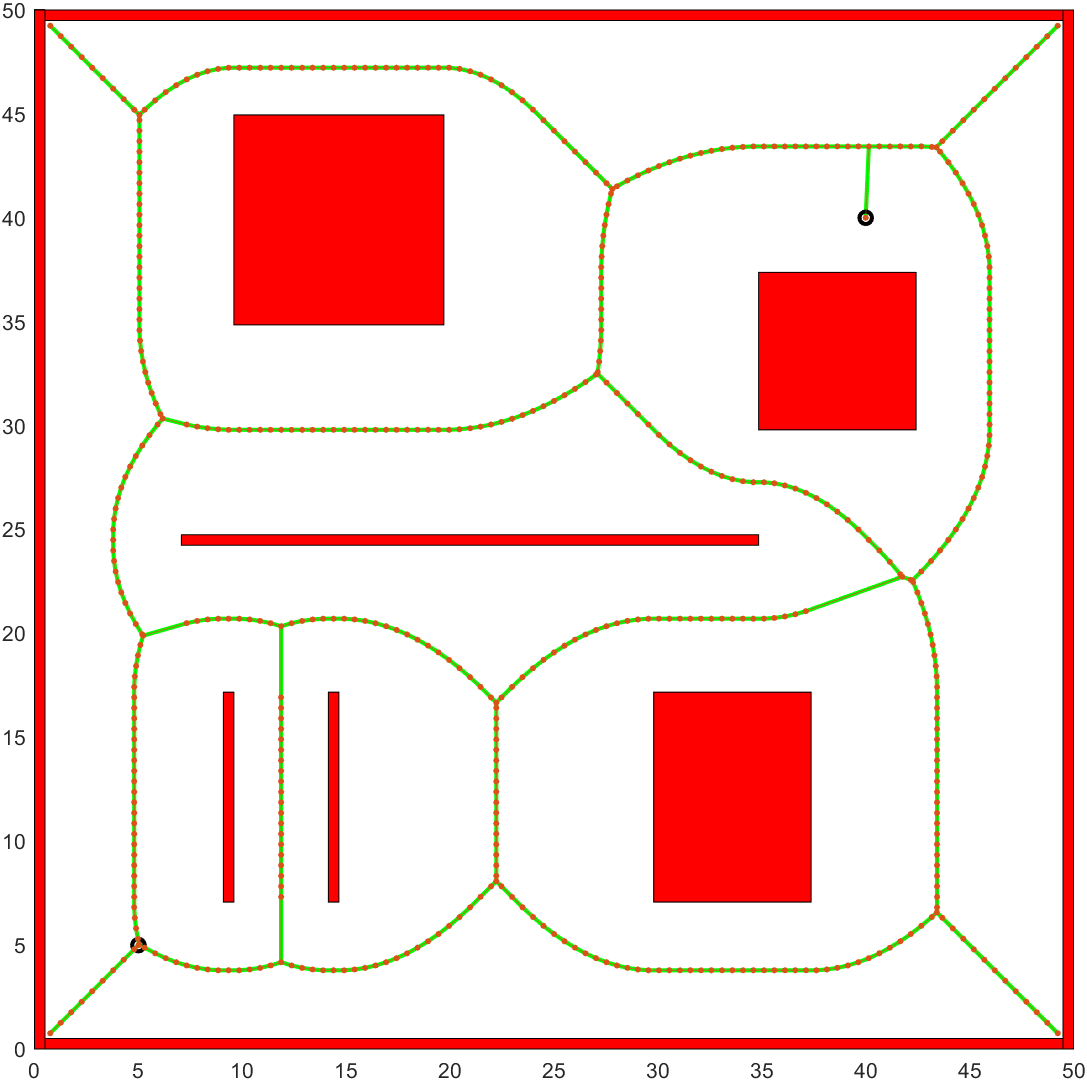
\includegraphics[width=\textwidth]{voronoi.png}
\label{voronoi}
\end{subfigure}
\hfill
\begin{subfigure}[t]{0.5\textwidth}
\centering
\caption{Decomposizione in celle}
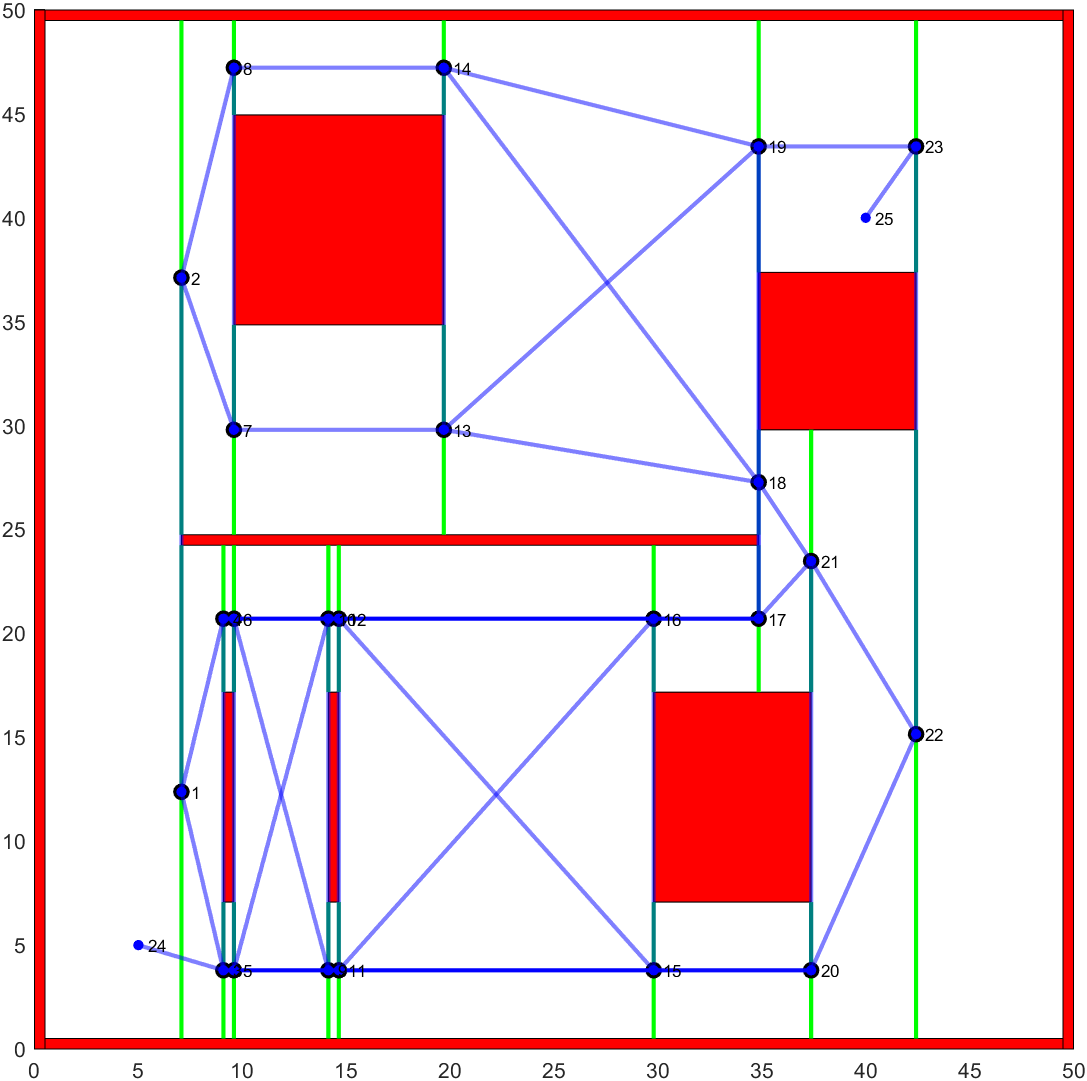
\includegraphics[width=\textwidth]{celldecomp.png}
\label{celldecomp}
\end{subfigure}
\caption{Metodi classici basati su grafo}
\end{figure}
Dunque, come appena visto, il path planning globale é ampiamente risolto grazie ai metodi appena descritti, tuttavia, sono particolarmente efficienti nel caso in cui ci si trovi in un ambiente noto a priori, poco incline al cambiamento e con l'esigenza di fare query ripetute. Il costo computazionale é quasi tutto contenuto nel calcolo del grafo, e la singola query ha un costo legato al numero di archi.\\
Come da titolo, il presente elaborato ha come obiettivo specifico quello di esporre un lavoro di progettazione, implementazione e simulazione di un algoritmo di path planning \textbf{locale} basato su \textbf{switching} tra \textbf{potenziali artificiali}. 

\subsection{Formalizzazione del problema} \label{problema}

Sia \( r(t) = [x_r(t),y_r(t),\theta_r(t)]^T\) la posizione del robot nell'istante t (per semplicità di notazione, ove necessario, si ometterà la dipendenza dal tempo nelle formule) e \( O_i(t) = [x_{O,i}(t),y_{O,i}(t)]^T, i = 1...N\) la posizione degli N ostacoli mobili.
\begin{nota}
\textbf{Ipotesi semplificative senza perdita di generalità}
\begin{itemize}
\item Si assume che \(t \geq 0\) e che l'istante di inizio sia sempre 0 visto che il sistema é assunto essere tempo invariante nelle sue caratteristiche principali (non vi é usura)
\item Si assume che gli ostacoli mobili siano di forma circolare (tutti con raggio \(R_i\)), poiché per un ostacolo di forma generica si può considerare la sua circonferenza circoscritta
\end{itemize}
\end{nota}
Esisterà inoltre un punto \(G = [G_x, G_y]\) che indica l'obiettivo del robot. Il problema che ci si pone, con riferimento al path planning, consiste nel voler raggiungere il punto \(G\) dalla posizione iniziale \(r(0)\), tenendo conto degli \(N\) ostacoli in movimento. Il robot é dotato di un raggio di visione di \(r_v\) metri, entro il quale é capace di rilevare un ostacolo. Inoltre, con l'ipotesi di rilevare gli ostacoli tramite il loro centro, si presuppone che valga la seguente condizione
\[\begin{Vmatrix}\begin{bmatrix} x_r(t)\\ y_r(t) \end{bmatrix} - O_j(t)\end{Vmatrix} \leq r_v \] ovvero \( R_i \leq r_v, \forall i\). Ciò vuol dire che nel momento in cui il robot incontra un ostacolo, il centro di quest'ultimo é incluso in \(R_v\) e non vi è rischio di collisione ancor prima che l'ostacolo venga rilevato.

\subsection{Struttura dell'elaborato} 
Nella sezione subito dopo si parlerà del metodo dei potenziali artificiali e si motiverà la scelta di utilizzarli per il path planning.\\
Successivamente verrà affrontato l'algoritmo vero e proprio, per il quale é stato usato un approccio top-down nella progettazione e quindi anche nell'esposizione: verrà prima discusso, in una modalità ``bird-view", come é organizzato il software, affrontando come i diversi moduli interagiscono tra di loro per ottenere l'obiettivo finale, senza scendere in dettagli implementativi.\\
Dopo di che, sempre in una logica top-down, si affrontano (con riferimento alla figura \ref{arch}) i singoli moduli : per primo l'ambiente e come viene rappresentato, dopo di che il modulo di azione, poi pianificazione e infine percezione. Ogni modulo, quindi, viene trattato ipotizzando di avere già accesso al modulo ``inferiore" che gli fornisce dati in input. \\
I moduli, infatti, sono stati progettati e sviluppati indipendentemente gli uni dagli altri. Come si vedrà nella sezione 4, non vi é correlazione tra un modulo e l'altro, ma interagiscono tra di loro guidati da un oggetto - nel caso del presente elaborato sarà una classe che modella il Robot - che li incapsula tutti e che coordina le interazioni, senza curarsi della specifica implementazione sottostante. In questo modo é possibile sviluppare delle gerarchie indipendenti dei singoli moduli, con una enorme possibilità di riutilizzo e di adoperare diverse implementazioni, dalle quali la struttura del funzionamento ``ad alto livello" - per essere più specifici, il livello di astrazione a cui si trova la classe rappresentante il robot - non viene influenzata.

\newpage
\section{Potenziali artificiali}

Metodo introdotto per la prima volta negli anni 90 da Oussama Khatib, é tanto semplice quanto efficace per risolvere il problema del path planning. Si differenzia dai metodi precedentemente menzionati per il fatto che la traiettoria non viene costruita ``attivamente", nel senso che non vengono definiti dei punti di passaggio che formano una traiettoria ottimale. Piuttosto quello che si fa é, mediante l'interazione con i cosiddetti potenziali artificiali, cercare una \textbf{configurazione ottimale}. Quindi, la traiettoria viene costruita mentre il robot si muove, motivo per cui é un metodo adatto al path planning locale.

\subsection{Metodo classico}
Tradizionalmente, nel path planning basato su potenziali artificiali il robot viene fatto muovere mediante una funzione in due variabili, ovvero un potenziale scalare, che nasce dalla somma di due potenziali: attrattivo e repulsivo. Questi due potenziali sono chiamati artificiali perché generano una forza che guida il robot in ogni sua configurazione \(r\), nonostante nella realtà non vi sia nessuna sorgente a generare quella forza. Nello specifico, la forza generata dal potenziale é il suo antigradiente, ovvero il gradiente cambiato di segno, che indica al robot la direzione di moto localmente più promettente\cite{oriolo}, cioè verso il punto di minimo della funzione. Di conseguenza il potenziale attrattivo assume una forma tale da avere un unico punto di minimo posizionato proprio nel punto di arrivo, mentre il repulsivo ha un unico punto di massimo corrispondente alla posizione dell'ostacolo. Nello specifico, ciò é di solito realizzato grazie alla funzione della configurazione del robot
\[
e(r) = G - \begin{bmatrix} x_r(t)\\ y_r(t) \end{bmatrix}
\]
che misura l'errore tra la posizione del robot e il goal. L'idea dietro al potenziale attrattivo é di generare una funzione che sia direttamente proporzionale a \(e(r)\), e quindi assuma valori elevati lontano dal goal e valori bassi vicino al goal, creando così un punto di minimo nel goal stesso.

\begin{description}
\item[Il potenziale attrattivo] ha di solito la forma mostrata in figura \ref{potA}, in cui il punto di minimo, ovvero il goal, ha coordinate \([1,1.5]\). La funzione corrispondente é
\[
U_{a1}(r,G) = \frac{1}{2} \cdot k_1 ||e(r)||^2
\]
\begin{figure}[H]
\centering
\caption{Potenziale attrattivo di forma paraboloide}
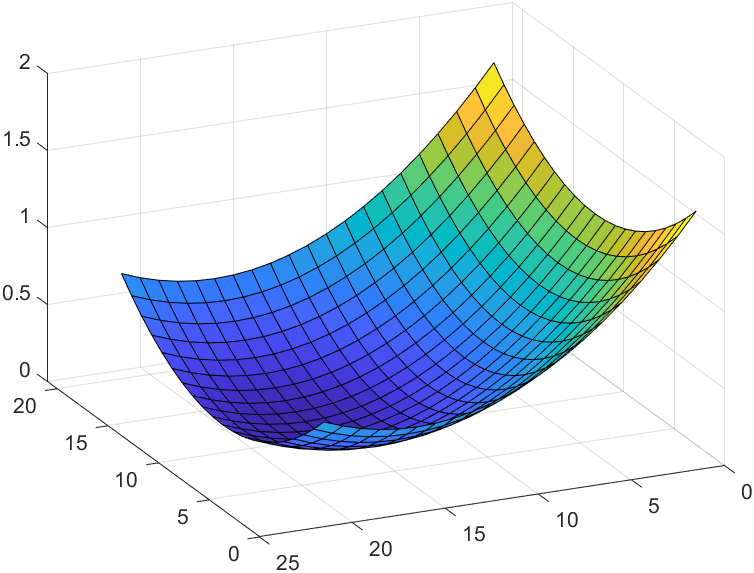
\includegraphics[width=0.8\textwidth]{potA.png}
\label{potA}
\end{figure}
Il suo antigradiente di conseguenza é formato da tanti vettori che, con un'intensità proporzionale alla distanza dal goal, puntano verso quest'ultimo.
\begin{figure}[H]
\centering
\caption{Antigradiente del potenziale attrattivo}
\label{antigradA}
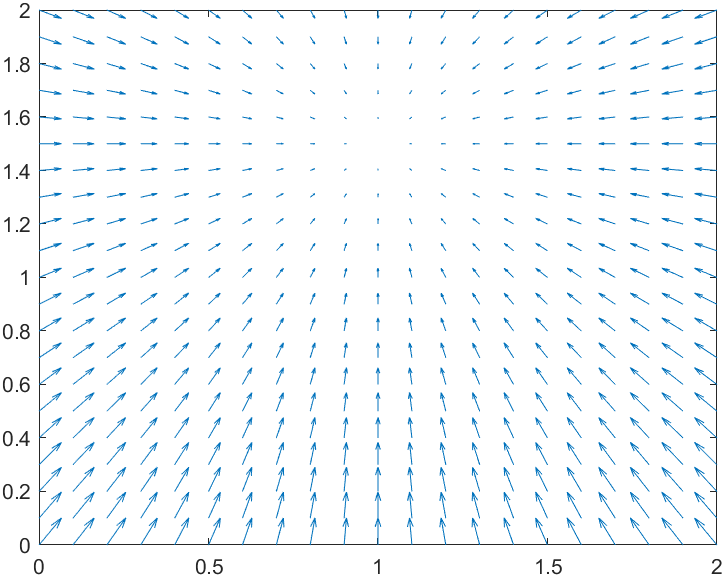
\includegraphics[width=0.6\textwidth]{antigradA.png}
\end{figure} 
Matematicamente si esprime come il vettore delle derivate parziali (del potenziale) cambiato di segno, ovvero 
\begin{equation}
-\nabla U_{a1}(r,G) = k_1 e(r)
\end{equation}
Perciò, la forza esercitata dal potenziale sul robot punta verso il goal e converge a zero quando la configurazione \(r(t)\) tende alla destinazione \(G\), esprimendo difatti l'errore tra goal e posizione del robot.\\

Oltre al potenziale paraboloide si può optare anche per un potenziale conico 
\begin{equation}
U_{a2}(r,G) = k_2||e(r)||
\end{equation}
e, come si può anche vedere in figura \ref{potACon}, la riduzione dell'errore all'avvicinarsi del robot al goal non é più quadratica, ma lineare. Da ciò scaturisce un comportamento più ``smooth" lontano dal goal (la velocità é meno elevata rispetto al potenziale paraboloide). Tuttavia, vicino al goal é conveniente usare quest'ultimo, per raggiungere la posizione esatta con minore velocità, il che conferisce più precisione al movimento del robot. 
\begin{figure}[H]
\centering
\caption{Potenziale attrattivo di forma conica}
\label{potACon}
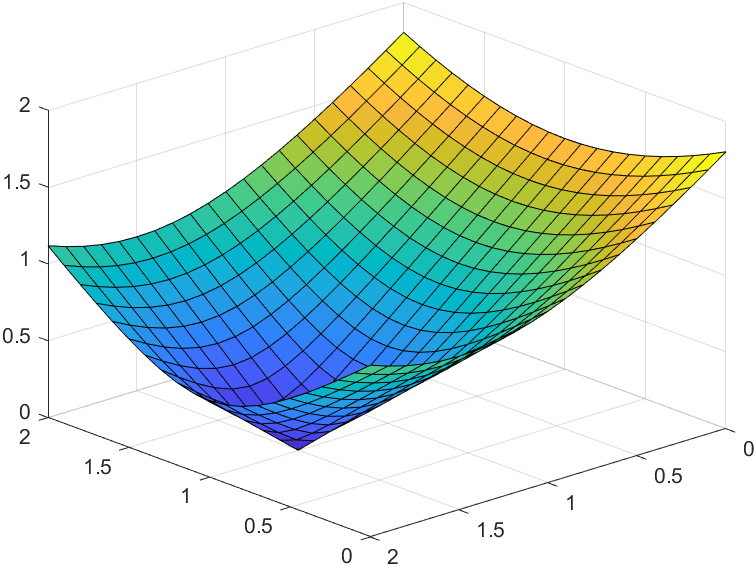
\includegraphics[width=0.8\textwidth]{potACon.png}
\end{figure}
L'antigradiente del potenziale conico ha la seguente espressione
\begin{equation}
-\nabla U_a(r,G) = k_2\frac{e(r)}{||e(r)||}
\end{equation}
L'idea é quella di stabilire una soglia per la funzione errore oltre la quale, avvicinandosi al goal, il potenziale attrattivo sarà di forma paraboloide. 
Dunque il potenziale attrattivo finale sarà del tipo
\begin{equation}
\label{potAC}
U_a(r) = 
\begin{cases}
\frac{1}{2} \cdot k_1 ||e(r)||^2 \quad &||e(r)|| \leq \rho \\
k_2||e(r)|| \quad &||e(r)|| > \rho
\end{cases}
\end{equation}

dove \(\rho\) é la soglia.  Gli scalari k e la soglia andranno scelti in maniera tale da garantire continuità nel passaggio da un potenziale attrattivo all'altro. In particolare deve valere che la velocità imposta dall'antigradiente al robot proprio nel punto di soglia deve essere la stessa per entrambi i potenziali, ovvero
\[k_1 \cdot e(r) = k_2 \cdot \frac{e(r)}{||e(r)||} \Leftarrow ||e(r)|| = \rho\]
da cui segue che 
\begin{equation}
\label{parconswitch}
k_1 \cdot \rho = k_2 
\end{equation}

\item[Il potenziale repulsivo] ha una forma duale a quello attrattivo, come mostrato in figura \ref{potR}. Esso impone che entro uno distanza \(\eta\) dall'ostacolo per il quale lo si sta calcolando, la sua funzione avrà valore inversamente proporzionale alla distanza dall'ostacolo stesso. Praticamente, più ci si avvicina all'ostacolo entro una certa soglia \(\eta\), più l'intensità del potenziale artificiale, perciò anche della forza generata da esso, aumenta.

\begin{figure}[H]
\begin{subfigure}[t]{0.5\textwidth}
\caption{Potenziale repulsivo}
\label{potR}
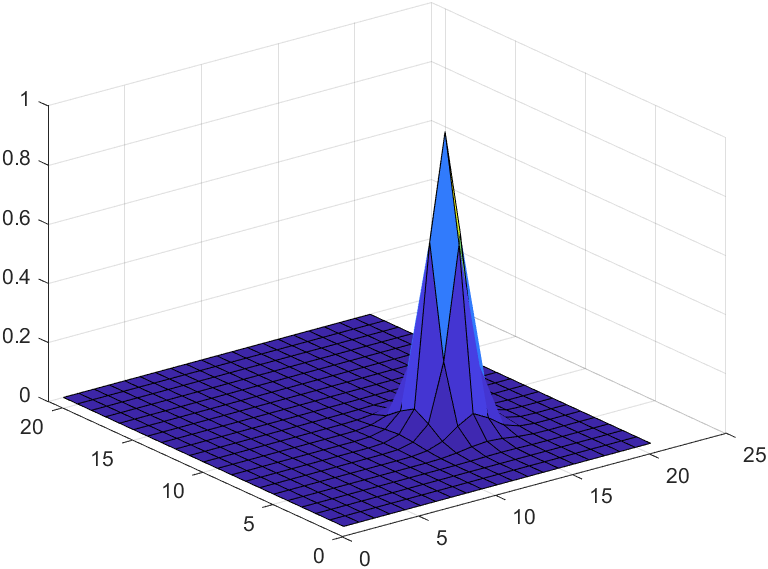
\includegraphics[width=\textwidth]{potR.png}
\end{subfigure}
\hfill
\begin{subfigure}[t]{0.5\textwidth}
\caption{Antigradiente del potenziale repulsivo}
\label{antigradR}
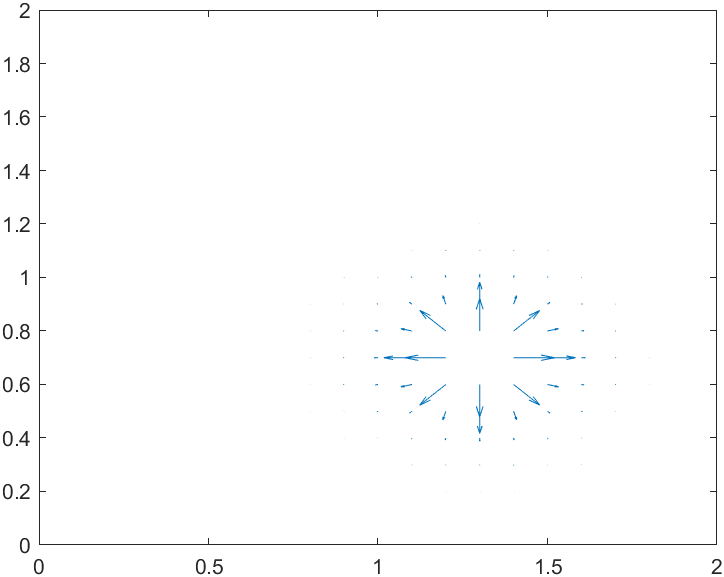
\includegraphics[width=\textwidth]{antigradR.png}
\end{subfigure}
\caption{Potenziale repulsivo}
\end{figure}

Al potenziale repulsivo corrisponde la seguente funzione a tratti 

\begin{equation}
\label{potREq}
U_r(r(t),O_j(t)) = 
\begin{cases}
\frac{1}{2} \left( \frac{1}{d(r(t),O_j(t)} - \frac{1}{\eta} \right) \quad &d(r(t),O_j(t)) \leq \eta \\
0 \quad &altrimenti
\end{cases}
\end{equation}
dove \[ d(r(t),O_j(t) = \begin{Vmatrix}O_j(t) - \begin{bmatrix} x_r(t)\\ y_r(t) \end{bmatrix}\end{Vmatrix}\]

Dunque, il compito della forza generata é quello di spingere via il robot dalla posizione dell'ostacolo tanto più che il robot si avvicina entro la soglia \(\eta\) a quest'ultimo. In figura \ref{antigradR} si vedono le linee di campo dell'antigradiente che puntano radialmente verso l'esterno rispetto alla posizione dell'ostacolo, qui con coordinate \([1.5, 1]\).
\end{description}
\paragraph{Potenziale totale}
A questo punto arrivati, una volta calcolato il potenziale repulsivo per ogni singolo ostacolo e il potenziale attrattivo legato al goal, si ottiene il potenziale totale:
\begin{equation}
\label{antigradeq}
U(r(t)) = U_a(r(t),G) + \sum_{j=1}^{n} U_r(r(t),O_j(t))
\end{equation}
In figura \ref{pot} si vede un possibile percorso del robot per arrivare dal punto di partenza al goal. \\
Dalla (\ref{antigradeq}) si vede che l'antigradiente è una funzione di \(r(t)\): vuol dire che in ogni sua configurazione, siccome l'antigradiente si suppone già calcolato prima ancora che il robot si metta in movimento, esso può ottenere informazioni sull'antigradiente riferendosi soltanto alla sua stessa posizione. Quindi, il vettore velocità del robot \([v_x(t) , v_y(t)]\) ha come riferimento in ogni istante t il valore dell'antigradiente (che é un vettore) in \([r_x(t),r_y(t)]\).\\
Lontano dagli ostacoli, il vettore velocità ha una direzione che punta al goal e un'intensità che diminuisce man mano che ci si avvicina al goal: più il robot si avvicina ad un ostacolo, più la direzione del vettore velocità vira verso il verso opposto rispetto a \(\theta = \tan \left( \frac{y_{O,j}(t)-y_r(t)}{x_{O,j}(t)-x_r(t)} \right) \) (la direzione del vettore che collega il robot all'ostacolo), spostando così temporaneamente la traiettoria desiderata e aumentando ``l'intensità della virata" lontano dall'ostacolo man mano che si avvicina ad esso. Il robot dunque, seguendo l'antigradiente, viene in ogni sua configurazione \(r(t)\) - usando l'analogia con il campo gravitazionale - attratto dal goal e \textbf{contemporaneamente} respinto dagli ostacoli.\\
Chiaramente, il metodo é idoneo sia al path planning globale che a quello locale (basta ricalcolare il potenziale totale in presenza di ostacoli). Volendo, d'altra parte, dare un'etichetta dal punto di vista dell'architettura di navigazione, i potenziali artificiali tradizionali obbediscono ad una di tipo reattivo: considerando la figura \ref{arch}, il modulo di mapping e path planning sono praticamente assenti. Gli attuatori del robot, che sono direttamente collegati ai sensori \cite{kim} e ricevono direttamente il comando derivante dal calcolo precedente del potenziale artificiale, senza alcun tipo di pianificazione algoritmica. 

\begin{figure}[H]
\centering
\caption{Potenziale totale}
\label{pot}
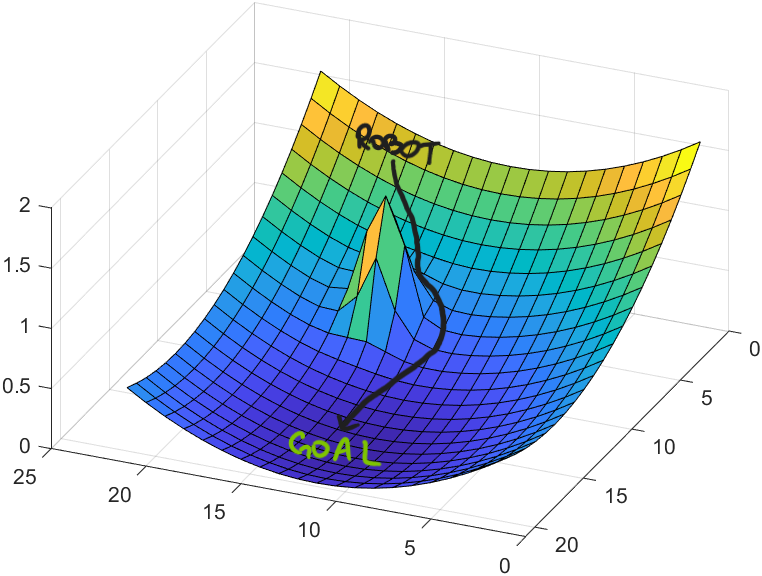
\includegraphics[width=0.7\textwidth]{pot.png}
\end{figure}
Tuttavia, nonostante la sua semplicità ed efficacia, vi sono delle non-idealità legate a questo approccio.\\
Ad esempio, la traiettoria potrebbe non essere continua. Il potenziale repulsivo non é ``coordinato" con quello attrattivo, perciò il robot potrebbe ricevere comandi che causerebbero un cambio di direzione o di velocità troppo repentino che andrebbe gestito dalla legge di controllo o un modulo di pianificazione apposito. Questa osservazione verrà approfondita meglio successivamente. \\
Altro problema da considerare é il fatto che il robot viene ``passivamente" spinto via dagli ostacoli senza la certezza che venga portato in una posa in cui può effettivamente evitare con successo l'ostacolo.\\
Ma il più importante, sicuramente, é il problema dei minimi locali: il robot non ha alcuna informazione su come uscirne, né può prevederli in anticipo. I minimi locali sono dei punti ad antigradiente nullo (il gradiente del potenziale attrattivo e repulsivo possono annullarsi a vicenda), dove il robot non ha nessuna forza a guidarlo verso il goal, situazione che dovrebbe verificarsi soltanto nel punto di goal stesso. In figura \ref{minloc} viene mostrato il percorso simulato di un robot in presenza di un minimo locale nel potenziale artificiale. Il robot parte dalla posizione \(r(0) = [5,0]\) mentre il goal si trova in posizione \(G = [5,10]\). Gli ostacoli sono posizionati tra il robot e il goal ad una distanza tale da causare un annullamento del gradiente (quindi il minimo locale) proprio a metà tra i due, lì dove il robot cerca di passare. La traiettoria del robot, infatti, si ferma nel minimo locale: non viene spinto da nessuna forza e ``crede" di essere arrivato nel punto di goal.
\begin{figure}[H]
\begin{subfigure}[t]{0.5\textwidth}
\caption{Potenziale con minimo locale}
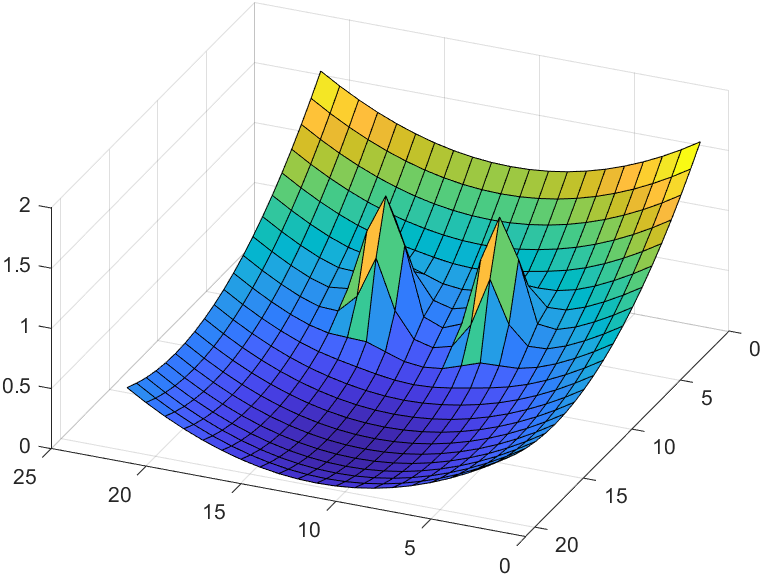
\includegraphics[width=\textwidth]{minimoLocale.png}
\end{subfigure}
\hfill
\begin{subfigure}[t]{0.5\textwidth}
\caption{Antigradiente del potenziale con minimo locale}
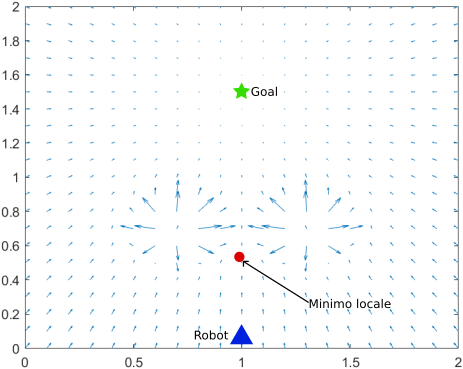
\includegraphics[width=\textwidth]{antigradMinimoLocale.png}
\end{subfigure}
\caption{Minimo locale}
\label{minloc}
\end{figure}

\subsection{Potenziale bypassante}
Al fine di evitare le non-idealità dovute all'utilizzo dei potenziali sommati, l'idea implementata nel presente elaborato é quella di sfruttare, per evitare gli ostacoli, al posto di quello repulsivo, un altro tipo di potenziale che verrà chiamato bypassante. Fondamentalmente, si tratta di un potenziale che invece di spingere via il robot dall'ostacolo, lo porta a circumnavigarlo. Infatti, le linee di campo dell'antigradiente di questo potenziale sono concentriche, al contrario di quelle del potenziale repulsivo che sono radiali. L'idea quindi é di basarsi su una superficie che ruoti attorno a un centro identificato da una certa coppia di coordinate, ad esempio un elicoide:
\[
\begin{cases}
x = x_0 + r cos(\xi) \\
y = y_0 + r sin(\xi)  \\
z = c \xi
\end{cases}
\]

Applicando nella terza equazione la tangente da entrambe le parti, otteniamo \(\tan(\xi)=\tan(\frac{z}{c})\) che, confrontando con le prime due equazioni, diventa
\[\tan \left( \frac{z}{c} \right) = \frac{y-y_0}{x-x_0}\] dove \([x_0,y_0]\) sarebbe la posizione dell'ostacolo. Invertendo questa funzione per esprimerla come z in funzione di x e y, otteniamo il potenziale elicoidale, ridenominato bypassante, in senso orario rispetto all'ostacolo e centrato in esso:

\begin{equation}
\label{potBeq}
\Gamma(x,y,x_0,y_0) = c\tan^{-1} \left( \frac{y-y_0}{x-x_0} \right)
\end{equation}

\begin{figure}[H]
\begin{subfigure}[t]{0.5\textwidth}
\caption{Elicoide centrato in \([1,1]\) \\ con \(c=2\), \(0\leq r \leq 1\) e \(0 \leq \xi \leq 4\pi\)}
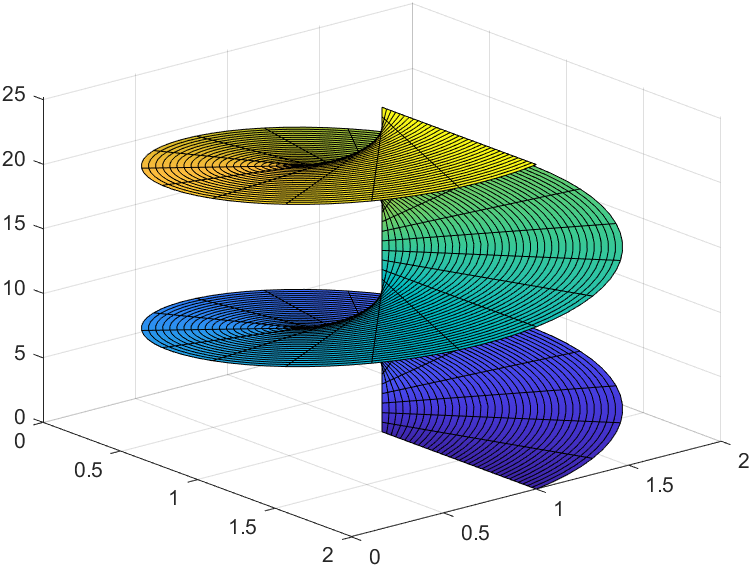
\includegraphics[width=\textwidth]{elicoide.png}
\end{subfigure}
\hfill
\begin{subfigure}[t]{0.5\textwidth}
\caption{Potenziale bypassante centrato in \([1,1]\) con \(c=2\) e in senso orario}
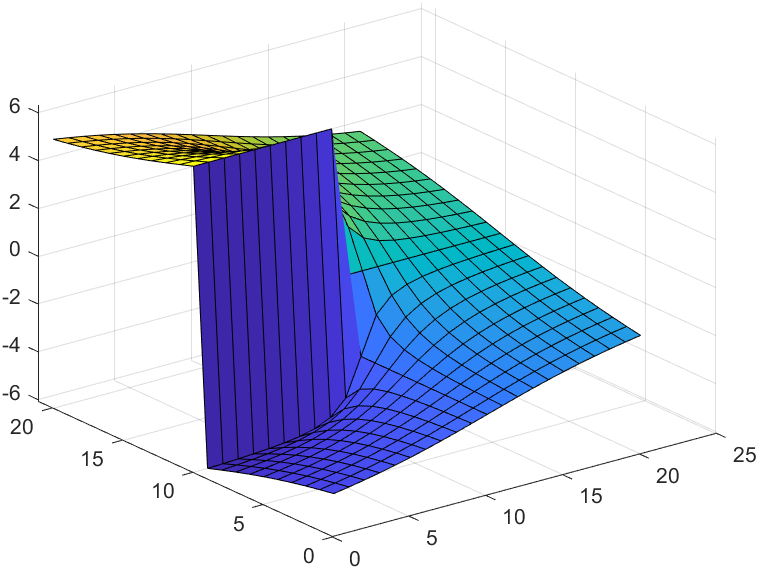
\includegraphics[width=\textwidth]{potB.png}
\label{potB}
\end{subfigure}
\caption{Potenziale bypassante}
\end{figure}

Da notare che il potenziale in figura \ref{potB} ha una discontinuità per \(x=x_0\), ma  la funzione in (\ref{antigradBeq}) é continua per \((x,y) \neq (x_0,y_0)\). Siccome il robot non può mai andare esattamente nella stessa posizione dell'ostacolo, non c'è perdita di generalità nell'ignorare la discontinuità e di conseguenza il robot sarà sempre in grado di seguire la forza generata dal potenziale. Il potenziale con equazione \ref{potBeq} può essere visto come una funzione della posizione del robot e dell'ostacolo da aggirare \[\Gamma(x,y,x_0,y_0) = \Gamma(x_r(t),y_r(t),x_{O,j}(t),y_{O,j}(t))\] Dunque, la forza generata dal potenziale bypassante é esprimibile come il suo antigradiente

\begin{equation}
\label{antigradBeq}
-\nabla U_b(r(t),O_j(t)) =
\begin{bmatrix}
\frac{c(y_r(t)-y_{O,j}(t))}{(x_r(t)-x_{O,j}(t))^2 + (y_r(t)-y_{O,j}(t))^2} \\\\
\frac{c(x_{O,j}(t) - x_r(t))}{(x_r(t)-x_{O,j}(t))^2 + (y_r(t)-y_{O,j}(t))^2}
\end{bmatrix}
\end{equation}\\

Quindi, l'antigradiente é formato da tanti vettori che
\begin{itemize}
\item Indicano una velocità desiderata nella posa \(r(t)\) del robot, al fine di aggirare l'ostacolo preso in considerazione  \item Aumentano di intensità man mano che il robot si avvicina all'ostacolo
\item Hanno forma concentrica
\end{itemize}

\begin{figure}[H]
\centering
\caption{Antigradiente del potenziale bypassante}
\label{antigradB}
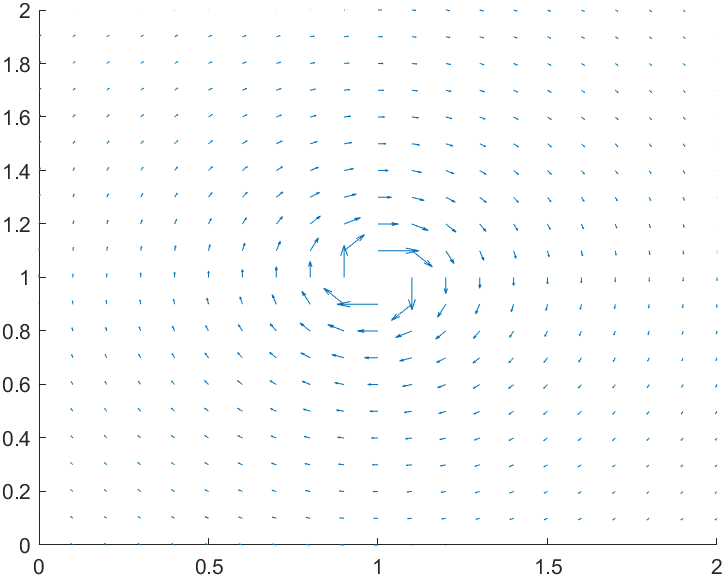
\includegraphics[width=0.8\textwidth]{antigradB.png}
\end{figure}

Questo tipo di potenziale, chiaramente, é intrinsecamente adatto ad ostacoli di forma circolare, motivo per cui nel lavoro di tesi si é considerato soltanto questo tipo di ostacoli.

\newpage
\section{Panoramica sull'algoritmo di navigazione} 
La strategia é semplice: nella posizione iniziale, il robot sonda l'ambiente attorno a sé. Le possibilità ora sono due:
\begin{itemize}
\item Non vi sono presenti ostacoli a impedirne l'avanzamento verso il goal, per cui la traiettoria da seguire é quella imposta dal potenziale attrattivo
\item Un ostacolo impedisce l'avanzamento del robot ed é necessario \textbf{``switchare"} dal potenziale attrattivo a quello bypassante, al fine di aggirare l'ostacolo, per poi tornare a seguire la traiettoria dell'antigradiente attrattivo
\end{itemize}
Perciò, la peculiarità di questo algoritmo é che in ogni istante di tempo il robot seguirà \textbf{un solo potenziale} alla volta, evitando così il problema dei minimi locali discusso in precedenza. Inoltre, le informazioni necessarie a pianificare lo switch non richiedono informazioni globali, ma solo di tipo \textbf{locale} relative all'ostacolo da aggirare. Nella figura \ref{flow} si vede, orientativamente, come funziona l'algoritmo. 

\begin{figure}[H]
\caption{Flowchart Diagram} \label{flow}
\centering
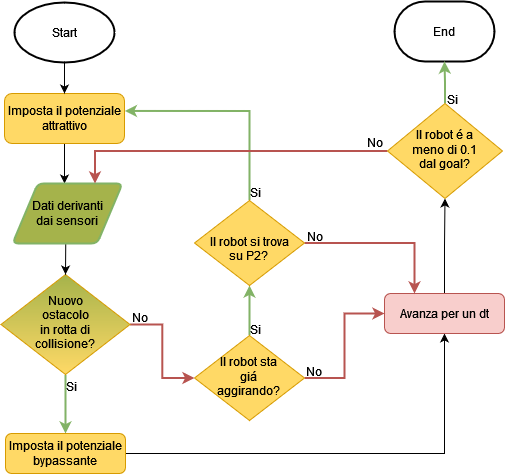
\includegraphics[width=0.7\textwidth]{flowchart.png}
\end{figure}

Le pseudo-istruzioni in giallo sono quelle relative al modulo di pianificazione e le verdi al modulo di visione. Naturalmente verranno approfonditi nelle rispettive sezioni (si spiegherà anche il significato del punto P2). Si vede qui ancora una volta la sequenza di azioni: prima interviene il modulo di percezione, che restituisce al modulo di pianificazione le informazioni visive e cognitive raccolte. Quest'ultimo a sua volta decide se impostare il potenziale attrattivo o bypassante in base ai due controlli al centro. Infine, il robot viene fatto muovere per un \(dt\), il che suggerisce che l'approccio alla simulazione é discretizzato. Ciò vuol dire il robot eseguirà in loop tutte le azioni del flowchart diagram ogni \(dt\).

\subsection{Architettura software}
\begin{figure}[H]
\centering
\caption{Class diagram}
\label{classdiagram}
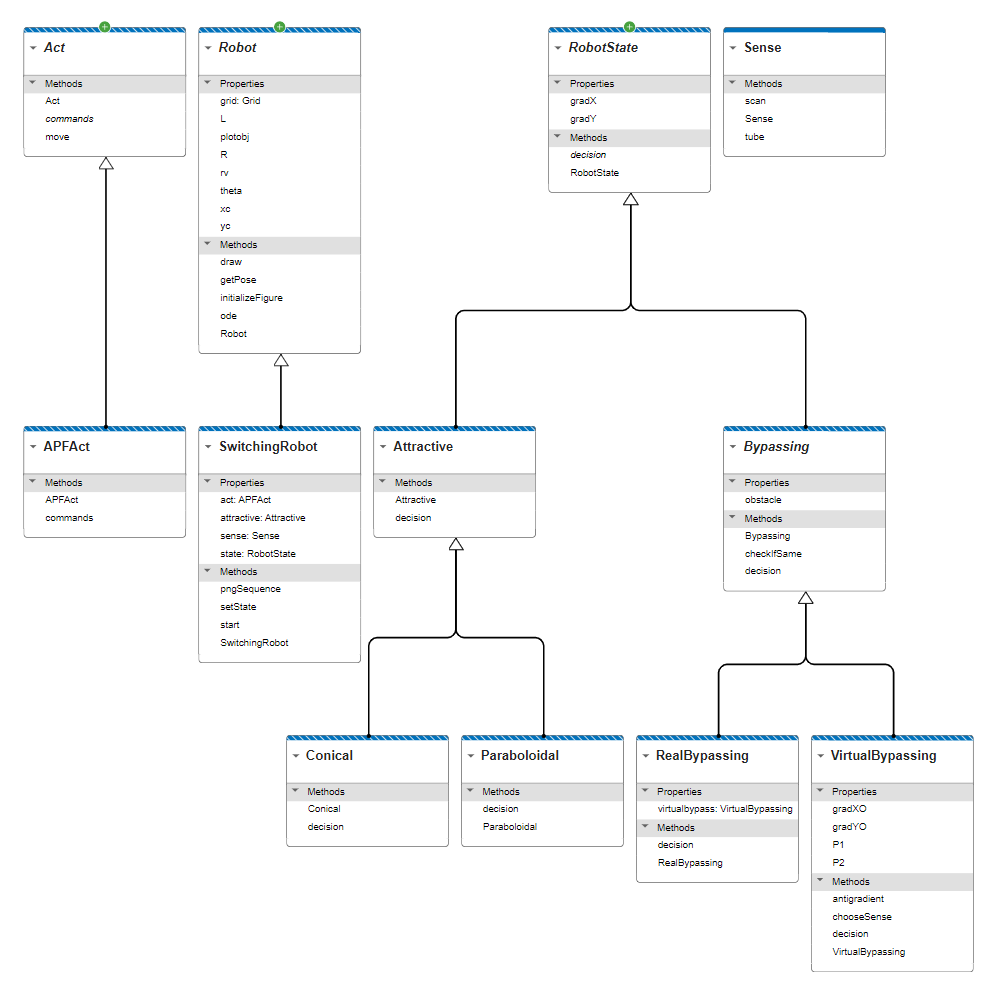
\includegraphics[width=\textwidth]{classDiagram.png}
\end{figure}
In figura \ref{classdiagram} é riportato il class diagram del software di navigazione. Le classi Act e Sense rappresentano rispettivamente il modulo di azione e pianificazione. Il modulo di pianificazione é costituito dalla gerarchia ``figlia" della classe astratta RobotState. SwitchingRobot é la classe che incapsula i tre moduli e ne fa uso all'interno di un suo ``main" che é il metodo start. Si può quindi notare che i tre moduli sono completamente disaccoppiati tra di loro e interagiscono soltanto tramite la classe SwitchingRobot.\\
Quindi, per capire meglio come le classi sono collegate tra di loro, nel seguente codice, che si trova appunto nella classe SwitchingRobot, é illustrato il funzionamento dell'algoritmo dal punto di vista del robot, che, come é facile vedere, é completamente disaccoppiato dalle implementazioni concrete dei singoli moduli di navigazione.
\begin{lstlisting}[caption=Entry point del modulo software, label=start]
function obj = start(obj)
	%Simulation data
	e = norm([obj.xc,obj.yc]-obj.grid.goal);
	tspan = 0.05; tsim = 0; samples = 0;
	%Starting simulation
	while(e > 0.1 && tsim < 20)
		%Sensed obstacle (empty array if nothing was sensed)
		dObstacle = obj.sense.scan(obj);
		%New directive
		obj.state.decision(obj,dObstacle);
		%Giving the command to the actuators 
		[obj.xc,obj.yc,obj.theta] = obj.act.move(obj,tspan);
		%Refreshing the error
		e = norm([obj.xc,obj.yc]-obj.grid.goal); 
		tsim = tsim + tspan; pause(0);
	end
end
\end{lstlisting}
L'idea é che il robot proceda in maniera discreta, ovvero che faccia dei campionamenti in istanti equidistanti e si muova di conseguenza. Fa da ``guida" il ciclo while, il cui ``indice di scorrimento" é l'errore \(e\) tra robot e goal. Questo ciclo si ripeterà naturalmente fino a che il robot non sarà arrivato nel punto di goal. Il tempo del ciclo é scandito dalla variabile \(tspan\), che indica il tempo tra un istante di campionamento e il successivo, dove con campionamento si intende, volgarmente, uno ``snapshot" dell'intorno da parte del modulo di visione. \\
Come si vede nel codice, il meccanismo attuato ad ogni iterazione é molto semplice: dapprima si controlla se é stato rilevato un ostacolo attraverso il metodo scan della classe Sense. Successivamente la variabile dObstacle, che é vuota se non viene rilevato nessun ostacolo, viene passata al metodo decision.\\
Quest'ultimo é richiamato su un oggetto di tipo RobotState. A seconda del sottotipo assegnato a RobotState, le azioni eseguite dal metodo decision saranno diverse (é proprio nel passaggio da uno un sottotipo di RobotState all'altro che avviene lo switch di potenziali).\\
Infine, una volta che il robot ha preso una decisione, passa il comando al modulo di azione per potersi effettivamente muovere attraverso il metodo move della classe Act (si parlerà meglio di questo metodo nella sezione sulla simulazione).\\ 
Si approfondirà nelle successive sezioni ognuna di queste tre ``macro-istruzioni" nel dettaglio, approfondendo cosa succede al loro interno.

\section{Rappresentazione dell'ambiente}
Prima di affrontare i moduli che guidano il robot nell'ambiente circostante, ha senso chiedersi, a questo punto, come questo possa esser rappresentato, soprattutto in relazione ai potenziali artificiali. La scelta fatta nel presente elaborato é stata quella di rappresentare l'ambiente in maniera completamente discretizzata. Ciò che lo circonda é per il robot una matrice (nel linguaggio di Matlab una meshgrid) in cui ogni cella corrisponde a un \(dx\cdot dy\) del mondo reale. Di conseguenza, il potenziale artificiale sarà una funzione che si concretizza in una matrice della stessa dimensione della meshgrid (il calcolo dell'antigradiente sarà affrontato nel modulo di pianificazione). Ogniqualvolta il robot voglia calcolare il valore dell'antigradiente in un punto di coordinate \([x,y]\), é necessario convertire queste in indici della meshgrid. Ciò viene fatto dal metodo coord2index della classe Grid.
\begin{lstlisting}[caption=Metodo che converte coordinate cartesiane in indici della meshgrid]
function index = coord2index(obj,point)
	index = zeros(1,2);
	% x coordinate goes into the column index
	floorx = floor(point(1));
	index(2) = (floorx + obj.dx*floor((point(1) - floorx)/
		obj.dx))*obj.resolution + 1;
	% y coordinate goes into the row index
	floory = floor(point(2));
	index(1) = (floory + obj.dx*floor((point(2) - floory)/
		obj.dx))*obj.resolution + 1;
	index = floor(index);
end
\end{lstlisting}

\begin{nota}
\textbf{Nota}\\ Si é scelto, in merito alla rappresentazione dell'ambiente, di non sfruttare una griglia di occupazione binaria per gli ostacoli. Questo rende il modulo di visione un po' ``fittizio", nel senso che esso fa lo ``snapshot" semplicemente andando a vedere la posizione degli ostacoli nella classe Grid, cosa che nella realtà non avviene. Questa semplificazione non provoca perdita di generalità, poichè basta, appunto, aggiungere una griglia di occupazione binaria accessibile dal modulo di visione tramite un sensore lidar. In ogni caso, ciò che é importante dell'implementazione discretizzata é il metodo per passare da coordinate reali a coordinate della meshgrid.
\end{nota}

\newpage
\section{Modulo di azione}
Il modulo responsabile per il movimento del robot riceve in input un comando dal modulo di pianificazione, ovvero l'antigradiente da seguire, e restituisce in output una ``traduzione" del comando in una velocità da imporre agli attuatori (tramite una legge di controllo), tenendo conto dello specifico modello cinematico del robot. 
\begin{figure}[h]
\centering
\caption{Modello Differential-Drive} 
\label{dd}
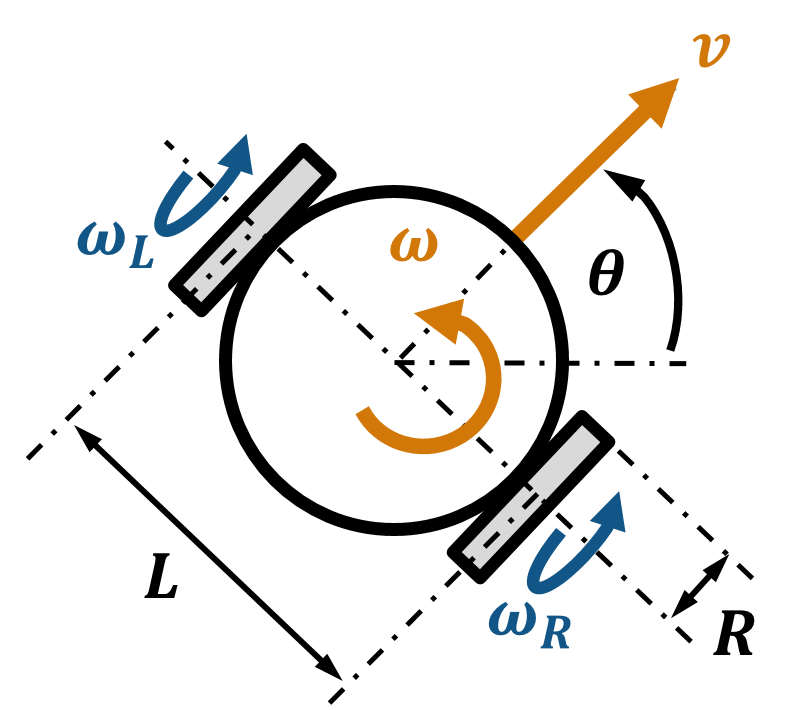
\includegraphics[width=0.8\textwidth]{DD.png}
\end{figure}

\subsection{Modello cinematico}
Si é ipotizzato in questa tesi di usare un modello cinematico anolonomo di tipo differential drive. Il fatto che sia anolonomo vuol dire che obbedisce ad un vincolo sulla velocitá e non sulla posizione, ovvero \[\theta(t) = \arctan \left( \frac{\dot{y}(t)}{\dot{x}(t)} \right) \] Praticamente, al robot é impossibile muoversi in ogni direzione con la stessa velocità; per mantenerla, deve continuare a mantenere il suo orientamento invariato. Le equazioni differenziali che modellano un generale robot che obbedisce a vincolo anolonomo é
\begin{equation}
\label{anolomeq}
\begin{cases}
\dot{x}(t) = v(t)\cos(\theta(t)) \\
\dot{y}(t) = v(t)\sin(\theta(t)) \\
\dot{\theta}(t) = \omega(t)
\end{cases}
\end{equation} 
Quindi, secondo questo modello, un robot può essere completamente caratterizzato mediante la sua posizione \([x,y,\theta]\) e la sua velocità \([v,\omega]\), dove \(v\) indica la velocità lineare (di traslazione) e \(\omega\) quella angolare (di rotazione).\\
In particolare, nel modello differential drive, il robot, come mostrato in figura \ref{dd}, viene mosso da due ruote laterali (ogni ruota ha il suo motore) di raggio \(R\), posizionate sullo stesso asse e distanti tra di loro \(L\).\\
Detto ciò, si può esprimere la velocità lineare come la media tra le velocità lineari delle due ruote \[v(t)=\frac{R\cdot\omega_R(t)+R\cdot\omega_L(t)}{2}\] e quella angolare come la differenza tra le due velocità lineari normalizzata per la distanza tra le ruote \[\omega(t)=\frac{R\cdot\omega_R(t)-R\cdot\omega_L(t)}{L}\] Riunite in forma matriciale, queste due relazioni danno la seguente
\begin{equation}
\begin{bmatrix}
v(t) \\
\omega(t)
\end{bmatrix}
=
\begin{bmatrix*}[r]
\frac{R}{2} & \frac{R}{2} \\
\frac{R}{L} & -\frac{R}{L}
\end{bmatrix*}
\begin{bmatrix}
\omega_R(t) \\
\omega_L(t)
\end{bmatrix}
\end{equation} 
Invertendo questa relazione, si può ottenere la velocitá delle due ruote a partire dalla velocità lineare e angolare di riferimento.
\begin{equation}
\label{wrwl}
\begin{bmatrix}
\omega_R(t) \\
\omega_L(t)
\end{bmatrix}
=
\begin{bmatrix*}[r]
\frac{R}{2} & \frac{R}{2} \\
\frac{R}{L} & -\frac{R}{L}
\end{bmatrix*}^{-1}
\begin{bmatrix}
v(t) \\
\omega(t)
\end{bmatrix}
\end{equation}
Questa inversione é sempre possibile, visto che
\[det\begin{bmatrix*}[r]
\frac{R}{2} & \frac{R}{2} \\
\frac{R}{L} & -\frac{R}{L}
\end{bmatrix*} = \frac{-R^2}{L}\] che é sempre non nullo, per cui la matrice é invertibile.\\
Dunque, il modello in equazione \ref{anolomeq} diventerá
\[
\begin{cases}
\dot{x}(t) = \frac{R}{2} \left( \omega_R(t)+\omega_L(t) \right) \cos(\theta(t)) \\
\dot{y}(t) = \frac{R}{2} \left( \omega_R(t)+\omega_L(t) \right)\sin(\theta(t)) \\
\dot{\theta}(t) = \frac{R}{L} \left( \omega_R(t)-\omega_L(t) \right)
\end{cases}
\]
La relazione appena ottenuta é implementata nella classe astratta Robot in quanto rappresentante del modello cinematico
\begin{lstlisting}[caption=Metodo che esprime lo specifico modello cinematico]
function [Xdot,wRwL] = ode(obj,vr,wr)
	K = [obj.R/2 obj.R/2 ; obj.R/obj.L -obj.R/obj.L];
	wRwL = K \ [vr ; wr];
	Xdot = 
	 ([cos(obj.theta) 0 ; sin(obj.theta) 0 ; 0 1] * K * wRwL);
end
\end{lstlisting}

\subsection{Legge di controllo}

Nel caso specifico del path planning con potenziali artificiali, la velocità di riferimento é data dall'antigradiente relativo alla posa del robot, cioè \(v_\nabla(t) = -\nabla U(r(t))\). Con la legge di controllo viene stabilita una velocità lineare e angolare da imporre al robot e viene stabilito che
\begin{equation}
v(t) = M_v \cos(\theta_{\nabla}(t) - \theta_r(t))
\end{equation} 
\begin{equation}
\omega(t) = K_{\omega}(\theta_{\nabla}(t) - \theta_r(t))
\end{equation} dove \(M_v=\begin{Vmatrix}v_{\nabla}(t)\end{Vmatrix}\), \(\theta_{\nabla}=\angle v_{\nabla}(t)\) e 
\[K_{\omega}(t)= \begin{cases}
\frac{\dot{\theta}_{\nabla}(t) + K_c|\theta_{\nabla}(t)-\theta_r(t)|^{\nu} \cdot sign(\theta_{\nabla}(t) - \theta_r(t))}{\theta_{\nabla}(t) - \theta_r(t)} \quad &|\theta_{\nabla}(t)-\theta_r(t)| \geq \xi \\
0 \quad &altrimenti
\end{cases}\]

Una volta calcolate le velocità di riferimento \(v(t)\) e \(\omega(t)\), basta applicare la relazione \ref{wrwl} per avere le velocitá di riferimento relative alle due ruote del differential drive, ottenendo cosí i comandi da impartire agli attuatori del robot.\\
La legge di controllo, specifica per questo metodo di navigazione, é implementata nel metodo commands. Quest'ultimo si trova nella classe APFAct (erede di Act) dove APF sta per artificial potential fields, il che vuol dire APFAct é idoneo a mobilitare tutti quei robot che sfruttano potenziali artificiali, indipendentemente dal modello cinematico. In output, il metodo commands restituisce le due velocità (lineare e angolare), che vengono poi convertite in altre due velocità (\((w_R\) e \(w_L)\) che sono gli effettivi comandi da attribuire ai motori che fanno girare le due ruote. In particolare, si possono notare due aspetti importanti:
\begin{itemize}
\item Le velocità desiderate (vGrad) sono, dopo aver prelevato gli antigradienti dallo stato attualmente in funzione del robot, calcolate nella posizione del robot tramite la funzione coord2index
\item \(\dot{\theta}_{\nabla}(t)\) viene calcolato per via numerica da riga 11 a 16
\end{itemize}

\begin{lstlisting}[caption=Metodo che genera i comandi di velocità]
function [vr,wr] = commands(~,rx,ry,rtheta,tspan,robot)
	grid = robot.grid; 
	gradX = robot.state.gradX; gradY = robot.state.gradY;
	i = grid.coord2index([rx,ry]);
	thetaN = atan2(gradY(i(1),i(2)),gradX(i(1),i(2)));
	thetaDiff = atan2(sin(thetaN-rtheta),cos(thetaN-rtheta));
	vgrad = [gradX(i(1),i(2)) gradY(i(1),i(2))];            
	Mv = norm(vgrad);
	vr = (Mv * cos(thetaDiff));
      
	rx1 = rx + vgrad(1)*tspan;
	ry1 = ry + vgrad(2)*tspan;
	j = grid.coord2index([rx1,ry1]);
	thetaN1 = atan2(gradY(j(1),j(2)),gradX(j(1),j(2)));   
	thetaDdiff = atan2(sin(thetaN1-thetaN),cos(thetaN1-thetaN));
	thetaDdot = thetaDdiff/tspan;
	
	Kc = 10; eps = 0.001; v = 1;
	Kw = (thetaDdot + Kc * abs(thetaDiff)^v * ...
	sign(thetaDiff))/(thetaDiff+eps);
	wr = (abs(thetaDiff) >= eps) * Kw * (thetaDiff);
end
\end{lstlisting}
La legge di controllo, così implementata, assicura che il robot converga alla velocità di riferimento \(v_{\nabla}(t)\) in un tempo finito \cite{dalfonso}.

\newpage
\section{Modulo di pianificazione}
Il modulo di pianificazione riceve ad ogni iterazione in input i dati processati dai sensori e in base a ciò decide a quale potenziale il robot deve fare riferimento, inoltrando successivamente la decisione al modulo di azione. 
\begin{nota}
\textbf{Nota implementativa} \\ Il modulo di pianificazione, argomento principe della tesi, é stato sviluppato indipendentemente dagli altri. Cioè, come preannunciato nella sezione \ref{problema}, si presuppone che il robot conosca in ogni istante la propria posizione e quella degli ostacoli all'interno del raggio di visione, come anche le loro velocità. Tale ipotesi semplificativa non provoca una perdita di generalità, grazie soprattutto al fatto che il software é stato progettato per essere modulare e con basso accoppiamento. Si parlerà meglio di questo aspetto nella sezione riguardante il modulo di visione.
\end{nota}
Data la struttura intrinseca dell'algoritmo di navigazione che si basa su un meccanismo di switching tra due stati, per definizione mutuamente esclusivi, un modo per modellare visivamente il pianificatore é sicuramente uno statechart diagram, come riportato in figura \ref{state}. Il robot può trovarsi, in una logica aut aut, nello stato corrispondente al potenziale attrattivo oppure in quello relativo al potenziale bypassante.

\begin{figure}[H]
\caption{Statechart Diagram} \label{state}
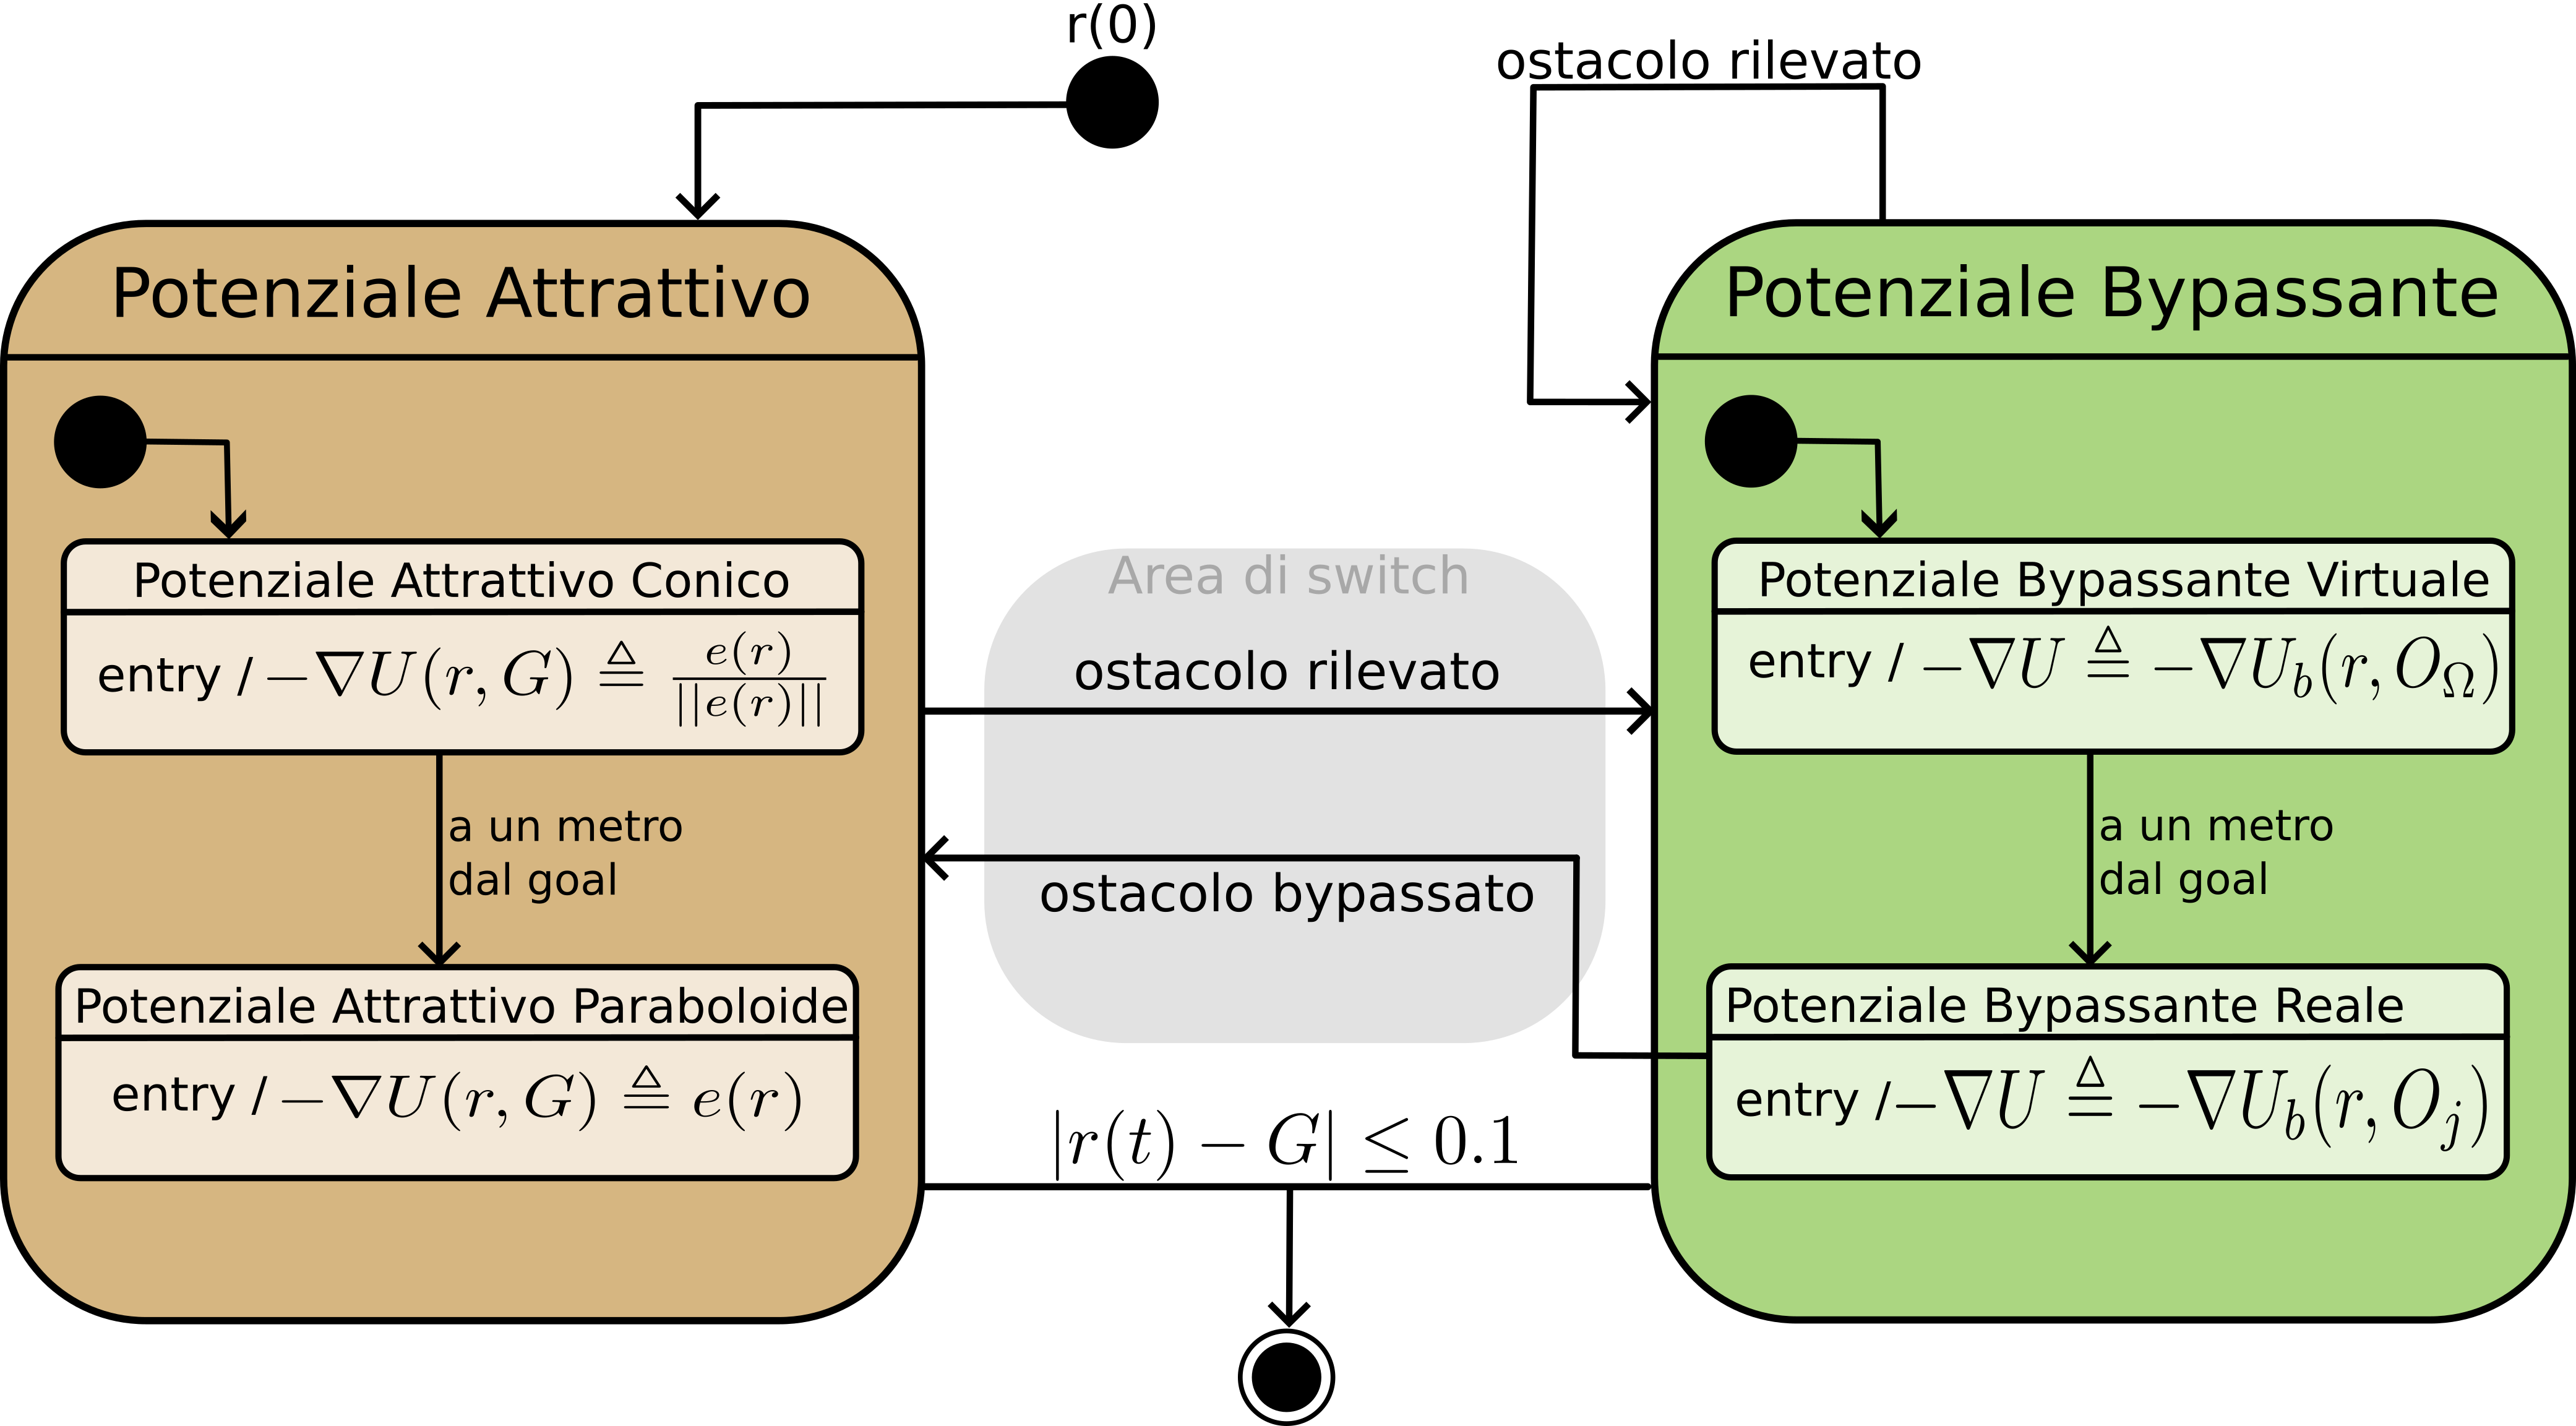
\includegraphics[width=\textwidth]{statechart.png}
\end{figure}

La strategia più naturale, sul piano dell'ingegneria del software, é di sfruttare il design pattern State per modellare correttamente il comportamento del robot. Ne consegue che gli oggetti di tipo SwitchingRobot hanno un campo RobotState che incapsula il comportamento relativo ad uno specifico antigradiente e quindi responsabile di gestire i comportamenti \textbf{state-specific}. Perciò, RobotState si configura come un'interfaccia che offre all'esterno il metodo decision (già visto nel metodo \ref{start}, il quale prende in input il robot e l'ostacolo rilevato. RobotState contiene anche l'antigradiente come variabile d'istanza: com'è naturale aspettarsi, ogni stato (attrattivo, bypassante ecc) possiede un specifico antigradiente. 
\begin{lstlisting}[caption=Classe asratta RobotState]
classdef (Abstract) RobotState < handle
    properties
        gradX; gradY;
    end
    
    methods (Abstract)
        obj = decision(obj,robot,dObstacle);
    end
end
\end{lstlisting}
Il metodo decision, in pratica, decide se operare o meno uno switch del campo state (riportato di seguito tra i campi della classe SwitchingRobot).
\begin{lstlisting}[caption=Campi della classe SwitchingRobot]
properties
	act APFAct = APFAct();
	sense Sense = Sense();
	state RobotState = DefaultRobotState();
	attractive Attractive;
end
\end{lstlisting}

\subsection{Stato attrattivo}
Lo stato iniziale del robot é quello attrattivo, conseguente all'imposizione del goal e il calcolo del potenziale attrattivo. Com'è prassi per il pattern State, ogni comportamento state-specific é incapsulato in una classe a parte. In questo caso specifico, la ridefinizione del comportamento specifico consiste nel ridefinire il metodo decision e calcolare gradX e gradY. Come riportato nel listing di seguito, se il robot si trova nello stato attrattivo, esso deve controllare innanzitutto se è stato rilevato un ostacolo, ed eventualmente prepararsi per bypassarlo. Il costruttore di VirtualBypassing é il metodo che calcola il potenziale bypassante e verrà trattato nel paragrafo successivo. Una volta calcolato il nuovo stato da assegnare al robot, viene richiamato il metodo setState che cambia il campo state dell'oggetto robot passato in input. 
\begin{lstlisting}[caption=Classe astratta Attractive (erede di RobotState)]
classdef Attractive < RobotState
	methods
		function obj = decision(obj,robot,dObstacle)
			if ~isempty(dObstacle)
				bypassing = VirtualBypassing(robot,dObstacle);
				bypassing.obstacle = [dObstacle.xc dObstacle.yc];
				robot.setState(bypassing);
			end
		end
	end
end
\end{lstlisting}
Come discusso nel capitolo sui potenziali artificiali, il potenziale attrattivo sarà conico fino a che \(e(r) > 1\). Infatti, vediamo che nel costruttore di SwitchingRobot, il potenziale attrattivo viene inizializzato a Conical.
\begin{lstlisting}[caption=Costruttore di SwitchingRobot]
function obj = SwitchingRobot(R,L,grid)
	obj@Robot(R,L,grid);
	obj.state = Conical(grid);
	obj.attractive = obj.state;
end
\end{lstlisting}
Nel costruttore di Conical é implementata l'equazione \ref{potAC} con \(k_2=1\). Quindi, nel momento in cui viene costruito l'oggetto SwitchingRobot, gli viene subito assegnato un potenziale attrattivo di tipo conico. L'implementazione a oggetti rende il software molto flessibile, poiché SwitchingRobot é indipendente dal potenziale che possiede. 
\begin{lstlisting}[caption=Costruttore di Conical]
function obj = Conical(grid)
	di = sqrt((grid.goal(1)-grid.X).^2 +
		 (grid.goal(2)-grid.Y).^2);
	obj.gradX = (grid.goal(1)-grid.X)./di; 
	obj.gradY = (grid.goal(2)-grid.Y)./di;
end
\end{lstlisting}
Nel caso del potenziale attrattivo conico vi sono due azioni da compiere: primo, eseguire l'implementazione di decision della classe padre di tutti i potenziali attrattivi (Attractive); secondo, controllare se il robot si trova a meno di un'unità di distanza dal goal ed eventualmente assegnare come stato quello paraboloide. La classe Paraboloidal si limiterà ad eseguire il metodo decision così come é stato ridefinito in Attractive.
\begin{lstlisting}[caption=Ridefinizione del metodo decision in Conical]
function obj = decision(obj,robot,dObstacle)
	decision@Attractive(obj,robot,dObstacle);
	rx = robot.xc; ry = robot.yc; grid = robot.grid;
	if norm([rx,ry]-grid.goal) < 1
		newattractive = Paraboloidal(grid);
		robot.attractive = newattractive;
		robot.setState(newattractive);
	end
end
\end{lstlisting}

\subsection{Switching allo stato bypassante}
Il costruttore di VirtualBypassing (si spiegherà successivamente perché il prefisso Virtual), fulcro di tutto il progetto, ha la responsabilità di calcolare il potenziale bypassante e tutto ciò di necessario affinché il robot sia in grado di giungere in una posa in cui non collida con l'ostacolo; nel linguaggio dello statechart costituisce la entry action del macrostato ``Potenziale Bypassante" in figura \ref{state}. L'obiettivo ultimo del metodo, perció, é di scambiare il potenziale correntemente in uso con quello bypassante. Naturalmente, il bypassing viene fatto con una ratio che si basa sulla velocità e la direzione di movimento dell'ostacolo da aggirare; in particolare, gli aspetti cardine da considerare sono:
\begin{itemize}
\item La scelta del verso di bypassing
\item Nessuna discontinuità nella traiettoria dovuta allo switch tra i potenziali
\end{itemize}

\paragraph{Primo aspetto}
La scelta del verso di bypassing é cruciale per una buona riuscita senza collisioni. Le possibilità, naturalmente, sono due: orario e antiorario.
\begin{lstlisting}[caption=Calcolo del verso di bypassing (orario o antiorario)]
xr = pose(1); yr = pose(2); thetar = pose(3); 
phi = atan2(obstacle.yc - yr,obstacle.xc - xr);
%Scelta verso
Rphi = [cos(phi-pi/2) cos(phi) ; sin(phi-pi/2) sin(phi)];
vphi = Rphi*obstacle.v;
if cos(atan2(vphi(2),vphi(1))) > 0
	sense = "clock";
else
	sense = "counterclock";
end
\end{lstlisting} 
La variabile phi indica l'angolo tra robot e ostacolo. Rphi, invece indica una matrice di rotazione che adatta l'angolo a cui viaggia il robot al sistema di riferimento di phi.\\
Quindi vphi indica com'é orientata la velocità del robot rispetto all'angolo tra esso e l'ostacolo: se vphi sta nel primo o quarto quadrante, l'ostacolo va aggirato in senso orario, altrimenti antiorario. Dunque, informalmente, se l'ostacolo si muove a destra rispetto alla direzione del robot, bisogna girare alla sua sinistra per evitare una collisione.
\begin{figure}[H]
\caption{Scelta del verso di bypassing}
\centering
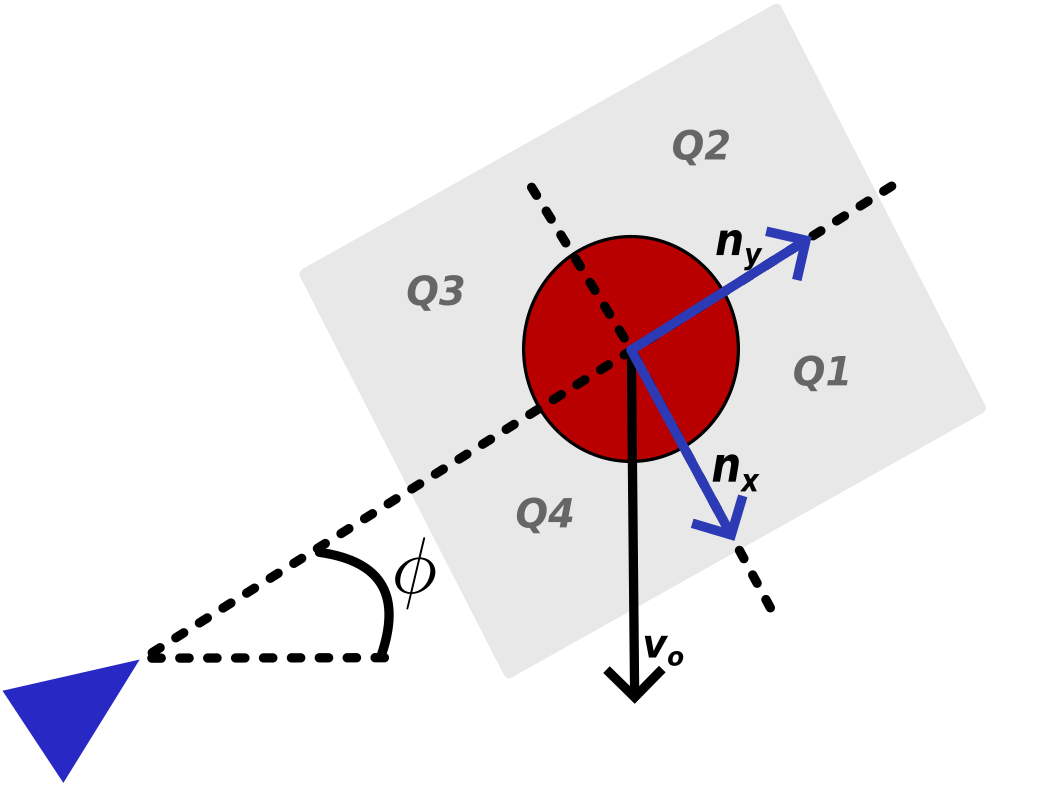
\includegraphics[width=0.7\textwidth]{sceltaverso.png}
\end{figure}

\paragraph{Secondo aspetto}
Lo scopo é quello di generare una traiettoria ``smooth", che sia in grado di assicurare continuità al moto del robot. Ci si pone quindi il problema di calcolare, nel momento in cui un ostacolo é stato rilevato, la velocitá e direzione di movimento del robot dopo lo switch. Nella pratica questo problema consiste, in prima battuta, nel calcolare il \textbf{punto preciso} in cui eseguire lo switch e il \textbf{coefficiente moltiplicativo} \(c\) - compare nell'antigradiente del potenziale bypassante in formula \ref{antigradB} - che modula la velocità di bypassing. Tuttavia, un'ulteriore problematica é data dalla possibilità che il potenziale di bypass possa \textbf{riaggiornarsi}, conseguentemente al fatto che l'ostacolo potrebbe essere ripetutamente ri-rilevato (dopo la prima volta); in quest'ottica l'ostacolo verrà comunque bypassato, ma il movimento del robot potrebbe essere soggetto a discontinuità involute o, in generale, comportamenti non del tutto predicibili a priori. \\
L'idea di fondo dietro la \textbf{soluzione} é di calcolare il potenziale bypassante nell'istante \(\tau\) in cui viene rilevato per la prima l'ostacolo e mantenerlo fisso per tutta la durata del bypass. Quindi \[-\nabla U_b \left( r(t) , O_j(t) \right) \Rightarrow -\nabla U_b \left( r(t) , O_j(\tau) \right) \]
\begin{nota}
\textbf{Nota} \\ Considerando questa strategia, potrebbe sorgere un problema nel caso in cui un ostacolo cambi direzione durante il bypass. Tuttavia, si é deciso, per scopi esemplificativi, di tralasciare questo aspetto, anche perché può essere gestito indipendentemente dalla struttura portante del modulo di pianificazione, con l'aiuto del modulo di visione.
\end{nota}
Una volta rilevato l'ostacolo nell'istante \(\tau\), il compito del pianificatore é di assegnare al robot un nuovo potenziale da seguire; questo, al fine di rendere continuo lo switch, sarà posizionato in un ostacolo virtuale e non, come ci si potrebbe aspettare, in quello realmente rilevato. La motivazione dietro a questo procedimento é la seguente. Le linee di campo del potenziale bypassante sono delle circonferenze. Il robot possiede in ogni istante una velocità, data da un vettore bidimensionale. Quindi, per far ``rientrare" il robot sul potenziale bypassante in maniera continua, bisogna trovare quella circonferenza che tange la traiettoria del robot nell'istante \(\tau\). La circonferenza cercata, in pratica, sarà una linea di campo del potenziale bypassante centrato nell'ostacolo virtuale. Solo successivamente il robot seguirà effettivamente il potenziale centrato nell'ostacolo reale. In figura \ref{circonferenze} é rappresentato lo scenario tipico nel momento in cui va bypassato un ostacolo. Il cerchio rosso interno rappresenta l'ostacolo, mentre il rosso esterno rappresenta la circonferenza centrata nell'ostacolo reale che rappresenta una sorta di ``delimitatore" oltre il quale non andare per non collidere con l'ostacolo. I cerchi blu e ciano indicano le (uniche) due alternative per il robot (come indicato anche dai numeri a pedice) e rappresentano le circonferenze centrate nell'ostacolo virtuale \(\Omega\); di conseguenza, la traiettoria che va dal robot a P1 rappresenta l'antigradiente del potenziale bypassante centrato in \(\Omega\), mentre quella da P1 a P2 l'antigradiente del potenziale bypassante centrato in \(r(\tau)\). Notiamo che la traiettoria é continua, senza punti di rottura o virate improvvise. Naturalmente, la continuità andrà gestita anche in termini di velocità del robot.

\begin{figure}[H]
\caption{Possibili percorsi dopo aver rilevato un ostacolo}
\label{circonferenze}
\centering
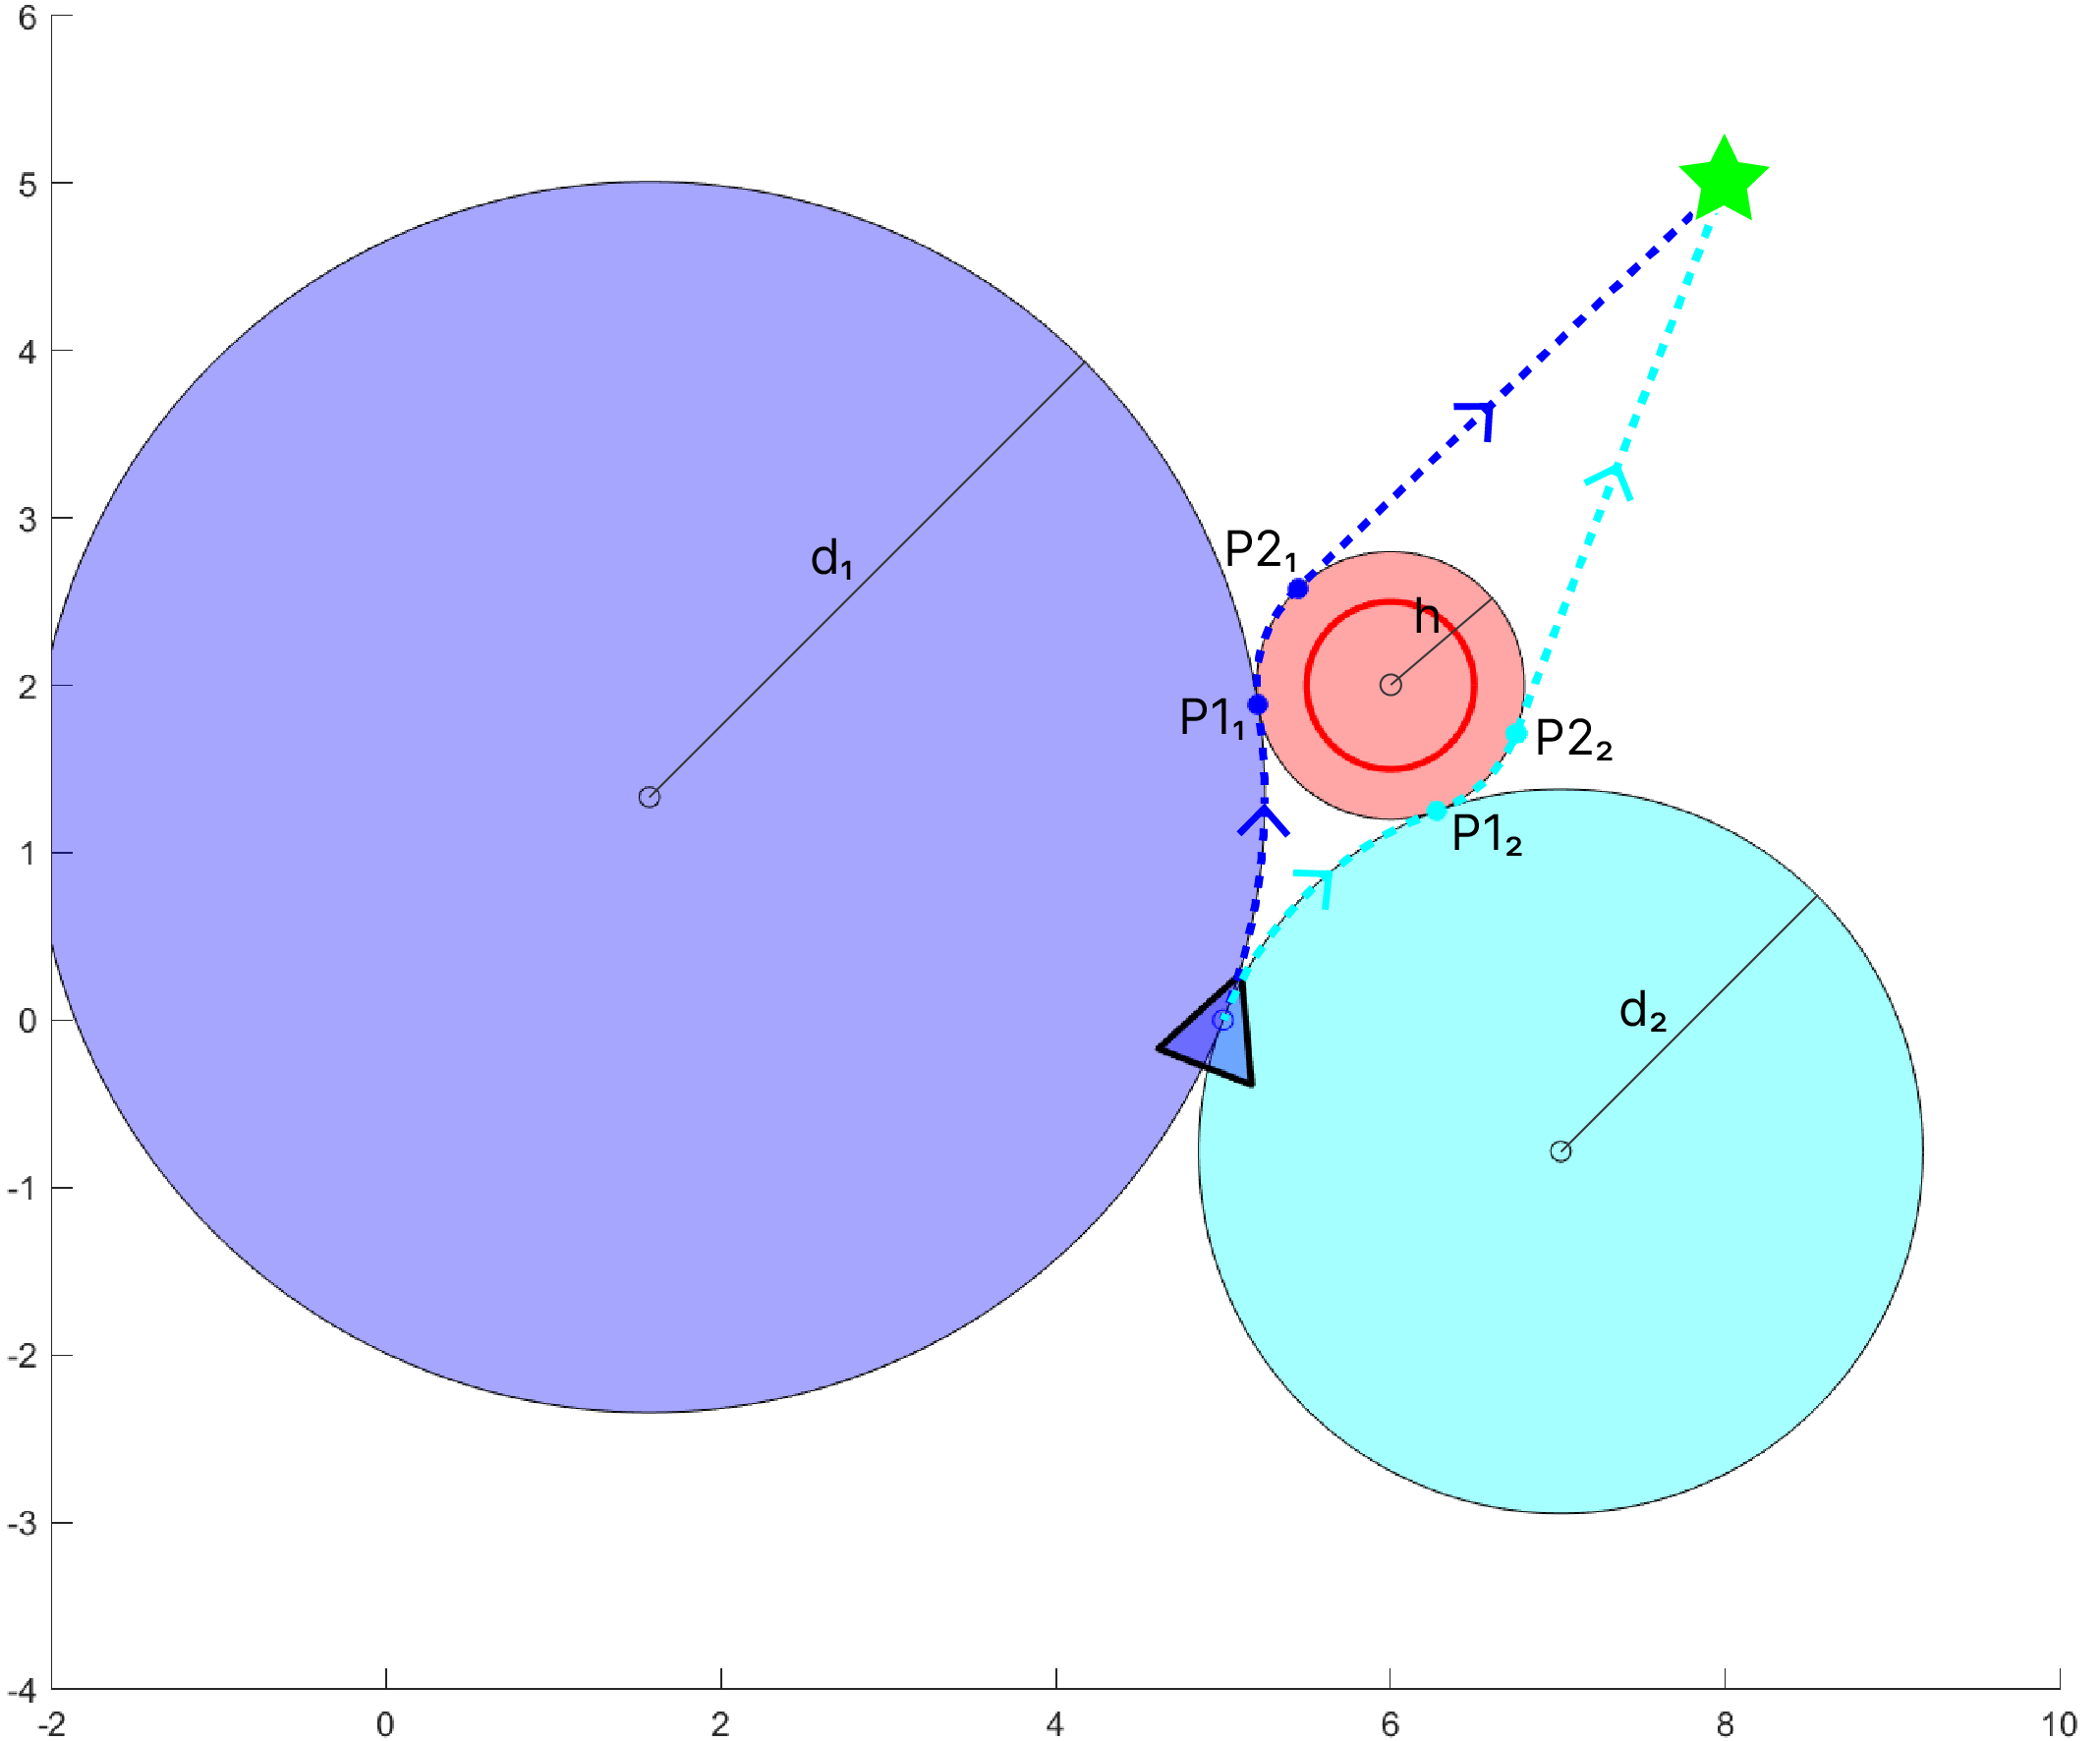
\includegraphics[width=\textwidth]{circonferenze.png}
\end{figure}

Più in dettaglio, gli ``ingredienti" del potenziale bypassante sono:
\begin{enumerate}
\item Posizione dell'ostacolo virtuale
\item Punto in cui switchare dall'ostacolo virtuale al reale (P1)
\item Punto in cui switchare dall'ostacolo reale al potenziale attrattivo (P2)
\item Coefficiente dell'antigradiente nell'ostacolo virtuale e reale
\end{enumerate}
Il primo punto si configura come un sistema di due equazioni in due incognite, ovvero \([x_{\Omega}, y_{\Omega}]\). Uno dei due vincoli é dato dalla condizione di tangenza tra la circonferenza centrata in  \([x_{\Omega}, y_{\Omega}]\) e la direzione di moto del robot in \(\tau\). A tal fine si può supporre, senza perdita di generalità, che il robot si trovi nell'origine all'istante \(\tau\). Da ciò ne deriva che l'equazione della circonferenza centrata in \([x_{\Omega}, y_{\Omega}]\) diventa \[d^2=x_{\Omega}^2+y_{\Omega}^2\] dove \(d\) é il raggio della circonferenza. La condizione di tangenza é soddisfatta se \[x_{\Omega} = -m\cdot  y_{\Omega}\] dove \(m = \tan(\theta_r)\), cioè la direzione di moto del robot. In pratica, questa equazione afferma che la retta, che congiunge il robot al punto \([x_{\Omega}, y_{\Omega}]\), deve essere perpendicolare a \(\tan(\theta_r)\). L'altro vincolo si ricollega al secondo punto della ``lista di ingredienti": bisogna imporre (con un ragionamento simile al primo vincolo) che la circonferenza ``omega" sia tangente alla circonferenza attorno all'ostacolo reale nel punto di switch tra i due potenziali bypassanti. Di conseguenza si impone che \[(x_{\Omega} - x_o)^2 + (y_{\Omega} - y_o)^2 = (d+h)^2\] dove \([x_o, y_o]\) é il centro della circonferenza nell'ostacolo e \(h\) il suo raggio. Riunendo i due vincoli in un sistema si ottengono le due equazioni in due incognite
\begin{equation}
\begin{cases}
x_{\Omega} = -m\cdot  y_{\Omega} \\
(x_{\Omega} - x_o)^2 + (y_{\Omega} - y_o)^2 = (\sqrt{x_{\Omega}^2+y_{\Omega}^2}+h)^2
\end{cases}
\end{equation}
Risolvendo questo sistema per \(y_{\Omega}\) si ottengono due possibili soluzioni
\begin{equation}
\label{yOmega}
\begin{cases}
y_{\Omega,1}=\frac{(-h^2 + x_o^2 + y_o^2)(m x_o - y_o + h\sqrt{m^2+1})}{2h^2m^2 + 2h^2 - 2m^2x_o^2 + 4mx_oy_o - 2y_o^2} \\\\
y_{\Omega,2}=\frac{-(-h^2 + x_o^2 + y_o^2)(m x_o - y_o + h\sqrt{m^2+1})}{2h^2m^2 + 2h^2 - 2m^2x_o^2 + 4mx_oy_o - 2y_o^2}
\end{cases}
\end{equation}
\(x_{\Omega}\) viene poi trovato per sostituzione. La scelta di una soluzione piuttosto che l'altra - in linea di massima, una sarà a sinistra dell'asse tra robot e ostacolo e l'altra sulla destra - dipenderà dal verso di bypassing (verrà affrontato successivamente, così come anche il calcolo di P1).\\
Una volta calcolata la posizione dell'ostacolo virtuale e del punto di switch tra ostacolo virtuale e reale, é necessario calcolare il punto P2 di switch tra il potenziale bypassante e quello attrattivo. L'idea per risolvere tale problema é di trovare, tra le infinitamente possibili, una retta che passi per il punto di goal e tanga la circonferenza centrata nell'ostacolo reale proprio in P2. Anche in questo caso le soluzioni possibili saranno due; quella idonea verrà scelta in base al verso di bypassing. Innanzitutto, il fascio di rette che partono dal punto di goal e passano dal punto cercato sono esprimibili come \[y-y_g = m(x-x_g)\] dove \(x\) e \(y\) sono le coordinate del punto P2 cercato. Inoltre, il punto P2 si troverà naturalmente sulla circonferenza centrata nell'ostacolo reale \[(x-x_o)^2+(y-y_o)^2=h^2\] e sostituendo in questa l'espressione della retta in funzione di \(y\), si ottiene un'equazione che esprime i possibili punti di intersezione tra la generica retta e la circonferenza	
\[(m^2+1)x^2 -2(x_o+m(y_o-y_g+mx_g)x + (y_o-y_g+mx_g)^2+x_o^2-h^2=0\]
Ovviamente ci sono troppe incognite per poter risolvere questa equazione, ma noi interessa la coppia di rette tale per cui esse sono tangenti alla circonferenza. Ciò equivale a imporre che il punto di intersezione sia uno solo e quindi che quest'equazione di secondo grado abbia una sola soluzione. La conseguenza é che troviamo i due coefficienti angolari ponendo a zero il delta dell'equazione\[(-2x_o - 2m(y_o+y_g+mx_g))^2 - 4(m+1)((y_o-y_g+mx_g)^2+x_o^2-h^2)=0\] e le due soluzioni saranno 
\[\begin{cases} 
m_1=\frac{(x_g-x_o)(y_o-y_g)+h\sqrt{-h^2+(x_g-x_o)^2+(y_g-y_o)^2}}{h^2-(x_g-x_o)^2} \\\\
m_2=-\frac{(x_g-x_o)(y_o-y_g)+h\sqrt{-h^2+(x_g-x_o)^2+(y_g-y_o)^2}}{h^2-(x_g-x_o)^2} 
\end{cases}\]
grazie alle quali é possibile trovare le due soluzioni per P2. \\
Infine, dopo aver trovato i primi tre ``ingredienti", manca il quarto, che serve a garantire continuità nello switch tra diversi potenziali. L'obiettivo perciò é di trovare per i due potenziali un coefficiente modulante in maniera tale che 
\begin{equation}
\label{vincolo1}
-\nabla U_b(P1,\Omega(t)) = -\nabla U_b(P1,O(t))
\end{equation} e anche 
\begin{equation}
\label{vincolo2}
-\nabla U_b(P2,O(t)) = -\nabla U_a(P2)
\end{equation} A parole, le velocità del robot tra antigradienti ``adiacenti" devono essere uguali nei punti di switch. Quello che si fa in pratica é sfruttare il vincolo dato dal modulo del potenziale bypassante calcolato partendo dall'equazione \ref{antigradBeq} 
\begin{equation}
\label{vincoloc}
||\nabla U_b|| = \frac{c}{\sqrt{(x-x_o)^2+(y-y_o)^2}}
\end{equation} dove \([x,y]\) é un punto incognito e \([x_o,y_o]\) la posizione dell'ostacolo.\\ 
Riassumendo il tutto, lo switch da potenziale attrattivo a potenziale bypassante avviene nei seguenti step, tutti facenti parte del costruttore di VirtualBypassing:
\begin{enumerate}
\item Calcolo del verso di bypass
\item Calcolo del raggio attorno all'ostacolo reale
\begin{lstlisting}[caption=Istruzioni per calcolare h]
Rtheta = 
	[cos(thetar-pi/2) sin(thetar-pi/2) ; cos(thetar) sin(thetar)];
vtheta= Rtheta*obstacle.v;
alphavtheta = atan2(vtheta(2),vtheta(1));
angdiff = 
	abs(atan2(sin(-pi/2-alphavtheta),cos(-pi/2-alphavtheta)));
rv = robot.rv; ro = obstacle.raggio;
minlim = 0.2; maxlim = 0.2;
hmin = ro+minlim; hmax = rv - maxlim;
gradoinv = abs(1-angdiff/(pi/2));
h = ((hmax-hmin)*gradoinv + hmin);
\end{lstlisting}
Per calcolare il raggio attorno all'ostacolo reale - misura orientativamente la soglia massima di avvicinamento durante il bypass all'ostacolo rilevato in \(\tau\) - si sfrutta una quantità che verrà battezzata \textbf{``grado di invasività"} dell'ostacolo. Tale quantità é misurata innanzitutto con la variabile angdiff, che contiene la differenza, in valore assoluto, tra la direzione di velocità dell'ostacolo \(\theta_o\)(riportato nel sistema d'orientamento della direzione del robot, similmente alla scelta del verso di bypassing) e \(\frac{-\pi}{2}\). Quest'ultimo angolo rappresenta il grado massimo di invasività: ad esempio, se il robot viaggia con un angolo di \(\frac{\pi}{2}\), l'ostacolo gli sbatterà contro molto più velocemente se \(\theta_o\) é opposto a \(\theta_r\). Il grado di invasività é minimo, invece, quando l'ostacolo viaggia ad un angolo retto rispetto al robot. Quindi 
\[
\begin{cases}
|1 - \frac{angdiff}{\frac{\pi}{2}}| = 0 \quad grado \ minimo \\
|1 - \frac{angdiff}{\frac{\pi}{2}}| = 1 \quad grado \ massimo
\end{cases}
\]
(questo valore é assegnato alla variabile gradoinv) e si può notare che \(h\) é proporzionale a questo grado, nel senso che vale la seguente relazione
\[
\begin{cases}
gradoinv = 0 \Rightarrow h = R_i + minlim \\
gradoinv = 1 \Rightarrow h = r_v - maxlim
\end{cases}
\]
dove minlim e maxlim sono scelti arbitrariamente e indicano quindi rispettivamente la soglia massima di avvicinamento all'ostacolo (non può esssere troppo lasca) e il raggio massimo (non può essere troppo grande per non dover far fare al robot curve troppo brusche). Dunque h é una funzione lineare esprimibile come 
\[h(gradoinv): [0,1] \rightarrow [hmin,hmax]\]
\item Calcolo soluzioni per l'ostacolo virtuale
\begin{lstlisting}[caption=Istruzioni per calcolare \(x_{\Omega}\) e \(y_{\Omega}\)]
load yOmega; yOmega = double(subs(yOmega(:)));
xOmega = -m*yOmega;
d = double(sqrt(xOmega.^2 + yOmega.^2));
\end{lstlisting}
yOmega é un vettore di due componenti e si ottiene applicando l'equazione \ref{yOmega}. Di solito una circonferenza sta alla sinistra rispetto a phi e l'altra a destra, ma può anche succedere, per eventualità legate alle condizioni di tangenza con la circonferenza, che entrambe le soluzioni consistano in circonferenze dallo stesso lato. A tal fine aiuta il prossimo passo.
\item Scelta circonferenza idonea
\begin{lstlisting}[caption=Istruzioni per scegliere la circonferenza idonea]
bool1 = abs(norm(xOmega))>0.01&&sign(xOmega(1))==sign(xOmega(2));
bool2 = abs(norm(yOmega))>0.01&&sign(yOmega(1))==sign(yOmega(2));
if bool1 || bool2 %Ho due circonferenze dallo stesso lato
	[~,indiceC] = min(d);
else %Non ho due circonferenze dallo stesso lato
	if oSense == "clock" %voglio la circonferenza sinistra
		indiceC = (sign(sin(angle)) == sign(xOmega(1))) + 1;
	else %voglio quella destra
		indiceC = ~(sign(sin(angle)) == sign(xOmega(1))) + 1;
	end
end
xOmega = xOmega(indiceC) + xr; yOmega = yOmega(indiceC) + yr;
dOmega = d(indiceC); xo = xo0; yo = yo0;
\end{lstlisting}
Da riga 1 a 4 si controlla se le due circonferenze calcolate si trovano dallo stesso lato, nel qual caso ce ne sarà sicuramente una con un raggio molto grande. Ciò succede quando, da un lato o dall'altro, i vincoli di tangenza non riescono ad essere soddisfatti, per cui il risolutore simbolico di Matlab calcola una circonferenza che tange quella centrata nell'ostacolo reale, ma internamente invece che esternamente, motivo per cui avrà un raggio grande. La soluzione é semplicemente prendere la più piccola tra le due circonferenze in questo caso. Se siamo, invece, nel caso ``ordinario", bisogna estrapolare la circonferenza d'interesse a seconda del verso di percorrenza dell'ostacolo. Ricordando che, nel calcolare la circonferenza dell'ostacolo virtuale, si é ipotizzato che il robot fosse nell'origine. In base a questo ragionamento, con l'ausilio della variabile angle che ribattezzerò \(\alpha\) che indica la direzione di viaggio del robot si può fare il seguente ragionamento: 
\[
\begin{cases}
\sin{\alpha} \geq 0 \cap clockwise \Rightarrow x_{\Omega} \leq 0 \\
\sin{\alpha} \geq 0 \cap anticlockwise \Rightarrow x_{\Omega} \geq 0
\end{cases}
\]
In sostanza, se il verso di bypassing é orario, serve la circonferenza sinistra, che sarà quella per cui \(x_{\Omega}\) é non negativo se l'orientamento del robot ``punta" verso il primo o secondo quadrante. Allo stesso modo si può ragionare per tutti gli altri casi.
\item Calcolo del punto P1
\begin{lstlisting}[caption=Istruzioni per calcolare P1]
centerDir = [xo,yo]-[xOmega,yOmega];
centerDir = centerDir/norm(centerDir);
obj.P1 = [xOmega yOmega] + dOmega*centerDir;
\end{lstlisting}
Una volta calcolata la posizione dell'ostacolo virtuale, bisogna trovare il punto di tangenza tra la circonferenza trovata e quella centrata nell'ostacolo reale. Ciò si fa semplicemente sfruttando la conoscenza del fatto che, quando due circonferenza si tangono, la retta che congiunge i due centri passa per il punto di tangenza.
\item Calcolo del punto P2
\begin{lstlisting}[caption=Istruzioni per calcolare P2]
obj.P2 = double(subs(solxp2(indiceP2)));
syms xp2; xp2 = obj.P2(1);
obj.P2(2) = double(subs(solyp2(indiceP2)));
\end{lstlisting}
La scelta della soluzione é basa sul verso di bypass: indiceP2 é pari a 2 se il verso é antiorario.
\item Calcolo del coefficiente modulante del potenziale bypassante reale
\begin{lstlisting}[caption=Istruzioni per calcolare il potenziale bypassante reale]
agradX = robot.attractive.gradX; 
agradY = robot.attractive.gradY;
j = grid.coord2index(obj.P2);
cO = norm([agradX(j(1),j(2)) agradY(j(1),j(2))])*h;
[obj.gradXO,obj.gradYO] = obj.antigradient(dO,grid,cO,oSense);
\end{lstlisting}
Per rendere continuo lo switch da potenziale bypassante (reale) a potenziale attrattivo deve valere il vincolo nell'equazione \ref{vincolo2}. Quindi, riprendendo l'equazione \ref{vincoloc}, bisogna imporre che il coefficiente modulante del potenziale bypassante nell'ostacolo reale sia \[c=||\nabla U_a(P2)||\cdot h\]. 
\item Calcolo del coefficiente modulante del potenziale bypassante virtuale
\begin{lstlisting}[caption=Istruzioni per calcolare il potenziale bypassante virtuale]
dr = sqrt((pose(1)-X).^2 + (pose(2)-Y).^2);
dp = sqrt((obj.P1(1)-X).^2 + (obj.P1(2)-Y).^2);
drp = sqrt((obj.P1(1)-pose(1))^2 + (obj.P1(2)-pose(2))^2);
k = grid.coord2index(obj.P1); 
i = grid.coord2index([pose(1) pose(2)]);
currgradX = robot.state.gradX;
currgradY = robot.state.gradY;
cr = norm([currgradX(i(1),i(2)),currgradY(i(1),i(2))])*dOmega;
cp = norm([obj.gradXO(k(1),k(2)),obj.gradYO(k(1),k(2))])*dOmega;
cV = cr*(dp/drp) + cp*(dr/drp);
[obj.gradX,obj.gradY] = obj.antigradient(vObstacle,grid,cV,vSense);
\end{lstlisting}
Per quanto riguarda il potenziale bypassante nell'ostacolo virtuale, i vincoli da imporre sono due: uno é quello espresso in equazione \ref{vincolo1} e l'altro é definibile come \begin{equation}
c(r(t)) = ||\omega||\cdot d
\end{equation} dove \(\omega\) é il potenziale che il robot segue in \(r(t)\), attrattivo o bypassante che sia, e \(d\) il raggio della circonferenza centrata nell'ostacolo virtuale. Bisogna dunque stabilire una funzione una funzione per \(c\) che rispetti entrambi i vincoli. Ciò che si é fatto nella pratica é stato basarsi sulla distanza dai punti ``estremi" del potenziale bypassante (nell'ottica del movimento che fa il robot) \(P1\) e \(r(\tau)\). Le variabili dr e dp esprimono le distanze dai punti calcolate sulla meshgrid e cr e cp indicano i coefficienti nei due punti (i primi riferiti a \(r(\tau\)), mentre drp indica la distanza tra i due punti. La funzione, al rigo 10, esprime i due vincoli richiesti: 
\[
\begin{cases}
dr=0 \Rightarrow c=cr \\
dp=0 \Rightarrow c=cp
\end{cases}
\]
\end{enumerate}
Le istruzioni appena elencate fanno tutte parte, in questa sequenza naturalmente, del costruttore di VirtualBypassing.
	
\subsection{Stato bypassante}
Una volta che é avvenuto lo switch tra potenziale attrattivo e bypassante, bisogna definire, ricollegandosi allo statechart in figura \ref{state}, il comportamento state-specific quando il robot sta bypassando un ostacolo.\\ Innanzitutto, anche mentre il robot sta bypassando, il modulo di percezione deve essere recettivo a nuovi ostacoli da, eventualmente, bypassare. Perciò, nella classe astratta Bypassing, il metodo decision é ridefinito in tal senso. Il metodo checkIfSame restituisce l'ostacolo ricevuto in ingresso invariato soltanto se questo é diverso dall'ostacolo attualmente in procinto di essere bypassato. A parole, dunque, se l'ostacolo rilevato é nuovo, decision della classe Bypassing fa uno switch (come se il robot  si trovasse in uno stato attrattivo) ad un nuovo stato bypassante relativo al nuovo ostacolo.\\
\begin{lstlisting} [caption=Classe astratta Bypassing (erede di RobotState)]
classdef (Abstract) Bypassing < RobotState
    
	properties
		obstacle; %ostacolo che sta per essere bypassato
	end
    
	methods
		function obj = decision(obj,robot,dObstacle)
			%Controllo se l'ostacolo rilevato e' diverso
			%da quello che sto bypassando
			dO = obj.checkIfSame(dObstacle);
			robot.attractive.decision(robot,dO);
		end
        
		function dO = checkIfSame(obj,dObstacle)
			%%Ostacolo non rilevato
			if isempty(dObstacle)
				obj.obstacle = []; dO = []; return;
			end
			%%Ostacolo rilevato
			%Ho ancora in vista l'ostacolo che sto bypassando
			if ~isempty(obj.obstacle)
			%Controllo se l'ostacolo rilevato e' lo stesso
				distance = 
					sqrt((obj.obstacle(1) dObstacle.xc)^2 +
					(obj.obstacle(2) - dObstacle.yc)^2);
				if abs(distance - norm(0.05*(dObstacle.v))) < 0.01
					dO = []; %SI
				else
					dO = dObstacle; %NO
				end
			end
			%Non ho piu in vista l'ostacolo che sto bypassando
			if isempty(obj.obstacle)
				dO = dObstacle;
			end
			%Aggiorno l'ostacolo corrente con quello rilevato
			obj.obstacle = [dObstacle.xc dObstacle.yc];
		end
	end
end
\end{lstlisting}
\begin{nota}
Da notare che, per controllare che due ostacoli siano uguali, si é fatto un controllo di tipo odometrico basandosi sulla velocità dell'ostacolo e la posizione del robot. Ciò potrebbe essere soggetto ad errori di misura poichè il robot (e gli ostacoli) nella realtà non é fermo. Tuttavia, considerando un tempo di campionamento abbastanza piccolo, si può in merito a ciò ipotizzare che il robot e gli ostacoli siano fermi tra uno ``snapshot" e l'altro.
\end{nota}
Ammesso che, invece, il robot non incontri nuovo ostacoli. Come detto precedentemente, l'ordine dei potenziali bypassanti é sempre virtuale e poi reale. 
\begin{lstlisting}[caption=Ridefinizione del metodo decision di VirtualBypassing]
function obj = decision(obj,robot,dObstacle)
	decision@Bypassing(obj,robot,dObstacle);
	if norm([robot.xc robot.yc] - obj.P1) < 0.1
		robot.setState(RealBypassing(obj));
	end
end
\end{lstlisting}
Dunque, il metodo decision ridefinito nella classe VirtualBypassing deve controllare a ogni iterazione che il robot non sia arrivato al punto P1; se così é, avviene uno switch al potenziale centrato nell'ostacolo rilevato nell'istante \(\tau\). Successivamente, si esegue ad ogni iterazione la ridefinizione di decision della classe RealBypassing. 
\begin{lstlisting}[caption=Ridefinizione del metodo decision di RealBypassing]
function obj = decision(obj,robot,dObstacle)
	decision@Bypassing(obj,robot,dObstacle);
	if norm([robot.xc robot.yc] - obj.virtualbypass.P2) < 0.1
		robot.setState(robot.attractive);
	end
end
\end{lstlisting}
Similmente, si controlla ad ogni iterazione che il robot non sia già arrivato nel punto P2, nel qual caso bisogna switchare al potenziale attrattivo. \newpage

\section{Modulo di percezione}
L'unico scopo del modulo di percezione relativamente a questo specifico lavoro di tesi é di controllare se gli ostacoli siano d'intralcio alla traiettoria del robot verso il goal. Si é fatto dunque un'importante ipotesi semplificativa che consiste nel supporre che il robot conosca in ogni istante la posizione, velocità e identità degli oggetti che deve evitare. Ciò é stato fatto per due motivi: primo, per concentrarsi sullo sviluppo del modulo di pianificazione; secondo, perché é sufficiente rimuovere queste ipotesi aggiungendo un modulo di visione (che lavora indipendentemente dall'algoritmo di pianificazione), che sia in grado, ad esempio, di fare object-tracking come anche riconoscerli. Lo stesso ragionamento si può fare per la propriocezione del robot - la percezione della sua posizione nell'ambiente - per la quale é sufficiente nel software un modulo che integri odometria e, eventualmente, sensori esterni per migliorare la precisione delle misurazioni.\\
Le funzionalità del modulo di percezione sono racchiuse nella classe Sense. Il metodo scan riceve in input il robot e controlla, tra gli ostacoli presenti, quali sono quelli posizionati entro un raggio rv dal robot e dentro un tubo direzionato dal robot al goal di larghezza rm. 
Figura tubo
\begin{lstlisting}[caption=Classe per il modulo di percezione]
classdef Sense
    
    methods
        %% Method that looks in a radius rv 
        %%and a tube T(t) if there are any obstacles
        function dObstacle = scan(obj,robot)
            rx = robot.xc; ry = robot.yc; rv = robot.rv;
            n = length(robot.grid.obstacles);
            distances = zeros(1,n) + inf;
            dObstacles = cell(1,n);
            for j = 1 : n
                o = robot.grid.obstacles(j);
                distance = norm([rx ry] - [o.xc o.yc]);
                if distance <= rv && obj.tube(robot,o)
                    dObstacles{j} = o;
                    distances(j) = distance;
                end
            end
            %Ostacolo tra quelli rilevati a distanza minima
            [~,pos] = min(distances);
            dObstacle = dObstacles(pos); dObstacle = dObstacle{1};
        end
    end
    
    methods(Access=private)
        %% Method that builds the tube T(t)
        function result = tube(~,robot,obstacle)
            pose = robot.getPose(); rx = pose(1); ry = pose(2);
            grid = robot.grid;
            G = grid.goal;
            
            rm = robot.rv + 1;
            angle = atan2(G(2)-ry,G(1)-rx);
            deltaX = rm/2*sin(angle); deltaY = rm/2*cos(angle);
            x1 = rx + deltaX; y1 = ry - deltaY;
            x4 = rx - deltaX; y4 = ry + deltaY;
            x2 = G(1) + deltaX; y2 = G(2) - deltaY;
            x3 = G(1) - deltaX; y3 = G(2) + deltaY;
            
            m14 = (y4-y1)/(x4-x1); q14 = m14*x1 - y1;
            if abs(m14) > exp(10)
                v14 = (obstacle.xc - x1);
            else
                v14 = (obstacle.yc - m14*obstacle.xc + q14);
            end
            
            m12 = (y2-y1)/(x2-x1); q12 = m12*x1 - y1;
            if abs(m12) > exp(10)
                v12 = (x1 - obstacle.xc);
            else
                v12 = (obstacle.yc - m12*obstacle.xc + q12);
            end
            
            m34 = (y4-y3)/(x4-x3); q34 = m34*x3 - y3;
            if abs(m34) > exp(10)
                v34 = (x4 - obstacle.xc);
            else
                v34 = (obstacle.yc - m34*obstacle.xc + q34);
            end
            
            if (angle >= 0 && angle <= pi/2) %first quadrant
                result1 = v14 >= 0;
                result2 = v12 >= 0; result3 = v34 <= 0;
            elseif (angle > pi/2 && angle < pi) %second quadrant
                result1 = v14 >= 0;
                result2 = v12 <= 0; result3 = v34 >= 0;
            elseif (angle >= -pi && angle <= -pi/2 || angle == pi ) %third quadrant
                result1 = v14 <= 0;
                result2 = v12 <= 0; result3 = v34 >= 0;
            else %fourth quadrant
                result1 = v14 <= 0;
                result2 = v12 >= 0; result3 = v34 <= 0;
            end
            result = result1 && result2 && result3;
        end
    end
end
\end{lstlisting}
\newpage

\section{Simulazione}
L'algoritmo é stato simulato in ambiente Matlab. A tal proposito viene qui ripreso il codice che costituisce il ``main" del modulo software. 
\begin{lstlisting}[caption=Entry point del modulo software]
function obj = start(obj)
	%Simulation data
	e = norm([obj.xc,obj.yc]-obj.grid.goal);
	tspan = 0.05; tsim = 0; samples = 0;
	%Starting simulation
	while(e > 0.1 && tsim < 20)
		%Sensed obstacle (empty array if nothing was sensed)
		dObstacle = obj.sense.scan(obj);
		%New directive
		obj.state.decision(obj,dObstacle);
		%Giving the command to the actuators 
		[obj.xc,obj.yc,obj.theta] = obj.act.move(obj,tspan);
		%Refreshing the error
		e = norm([obj.xc,obj.yc]-obj.grid.goal); 
		tsim = tsim + tspan; pause(0);
	end
end
\end{lstlisting}
Dei metodo scan e sense si é parlato ampiamente, ma non del metodo move della classe Act. Tale metodo prende in ingresso il robot e l'intervallo di campionamento della simulazione, restituendo in output la nuova posizione del robot. Il metodo move sostituisce quindi gli effettivi attuatori del robot in maniera tale da poter simulare il movimento del robot in assenza di un robot reale.
\begin{lstlisting}[caption=Metodo responsabile di far muovere il robot in simulazione]
function [xc,yc,theta] = move(obj,robot,tspan)
	rx = robot.xc;
	ry = robot.yc;
	rtheta = robot.theta;
	[vr,wr] = obj.commands(rx,ry,rtheta,tspan,robot);
	Xdot = robot.ode(vr,wr);
            
	rx2 = rx + tspan/2*Xdot(1);
	ry2 = ry + tspan/2*Xdot(2);
	rtheta2 = rtheta + tspan/2*Xdot(3);
	[vr,wr] = obj.commands(rx2,ry2,rtheta2,tspan,robot);
	Xdot = robot.ode(vr,wr);
            
	xc = rx + tspan*Xdot(1);
	yc = ry + tspan*Xdot(2);
	theta = rtheta + tspan*Xdot(3);
end
\end{lstlisting}
Come si vede nel listing, il metodo genera dapprima i comandi di velocità con il metodo commands (di questo metodo si parlerà meglio nella sezione riguardante il modulo di azione), con i quali genera una variabile Xdot - derivata numerica nella posa attuale del robot - attraverso il metodo ode specifico per ogni modello cinematico. In pratica, quello che si fa é integrare numericamente attraverso la derivata numerica Xdot, come si vede da riga 14 a 16. La posizione del robot tra un istante di campionamento é pari alla posizione attuale più il prodotto tra la derivata (istantanea) della posizione e l'intervallo di campionamento. Nello specifico, in questo metodo si é scelto di adottare una doppia integrazione numerica (Eulero esplicito), denominata anche metodo ``Runge-Kutta 2". \\
Una volta definito quali sono i componenti dell'algoritmo a livello macroscopico, si può vedere come si avvia la simulazione nel suo totale nel seguente script.
\begin{lstlisting}[caption=Istruzioni per avviare la simulazione]
grid = Grid(50,10);
grid.setGoal([6,9]);
%Obstacles and robot initial configuration
grid.addObstacle(Obstacle(2,4,[1;0]));
grid.addObstacle(Obstacle(10,6,[-1;0]));
grid.addObstacle(Obstacle(1.5,10,[0.5;-0.5]));
n = length(grid.obstacles);
r = SwitchingRobot(0.15,0.3,grid);
%Inizio simulazione
r.start();
\end{lstlisting}
Si vede dunque che viene prima generato un oggetto di tipo Grid, ovvero la struttura dati che serve a rappresentare l'ambiente circostante. Successivamente vengono ``immessi" gli ostacoli (i primi due parametri del costruttore indicano la posizione e il terzo la velocità). Dopo di che, viene costruito il robot (il primo parametro del costruttore indica il raggio in centimetri delle ruote, mentre il secondo la distanza tra le due ruote). Infine, viene avviato il metodo start, già trattato in precedenza e la simulazione ha inizio.
 
\newpage
\section{Risultati}
Nel testare l'algoritmo di path planning si é usata la seguente configurazione di parametri:
\begin{itemize}
\item Il raggio di visione \(R_v=1.5m\)
\item La dimensione degli ostacoli \(R_i=0.5m\)
\item Le soglie di avvicinamento \(minlim = 0.2m\) e \(maxlim=0.2m\)
\item La larghezza del tubo direzionato \(R_m=3m\)
\item I parametri della legge di controllo \(K_c=10, c=1, \xi=0.001\) 
\end{itemize}
L'algoritmo é stato testato con successo su varie configurazioni di diverso tipo; a titolo esempio se ne riporteranno alcune che riassumano un po' tutti i casi ``ordinari" e un'altra a parte in cui si fa un confronto con il metodo classico nell'ambito di un caso ``patologico" per quest'ultimo (i minimi locali).\\
Da notare che il sistema di riferimento cartesiano é espresso in metri.

\subsection{Tre ostacoli}
La configurazione di partenza é la seguente: i tre ostacoli all'istante iniziale sono \(O_1=[2,4]\) con velocità \(v_1=[1,0]\), \(O_2=[10,6]\) con velocità \(v_2=[-1,0]\) e \(O_3=[2.5,10]\) con velocità \(v_3=[-0.5,-0.5]\). In figura \ref{snapshot1} sono riportati due punti salienti della simulazione.I cerchi pieni indicano le circonferenze di ostacolo virtuale e reale nell'istante in cui l'ostacolo rilevato, le circonferenze vuote indicano gli ostacoli veri e propri.\\
In figura \ref{bypass1} é riportato il movimento del robot nelle varie istantanee della simulazione: il cerchio rosso pieno rappresenta la posizione dell'ostacolo \(O_1\) nel momento in cui viene rilevato; vediamo perciò che il robot gira a sinistra in maniera tale da bypassare l'ostacolo in senso orario per non collidere. Se, naturalmente, il verso scelto fosse stato quello antiorario, il robot avrebbe colliso. Inoltre, notiamo che il robot non si cura di informazioni sensoriali riguardanti gli altri ostacoli, che non influenzano il bypassing in atto.\\
In figura \ref{bypass3} notiamo che avviene il bypass dell'ostacolo \(O_3\). Tuttavia, mentre il primo bypass avviene nella maniera ``ordinaria" (switch da potenziale attrattivo a bypassante e di nuovo all'attrattivo), qui assistiamo ad uno switch da potenziale bypassante dell'ostacolo \(O_2\) (indicato dai cerchi pieni più trasparenti) al potenziale bypassante di \(O_3\), come voluto dall'algoritmo, che mantiene attivo il modulo di visione anche durante un bypass.

\begin{figure}[H]
\begin{subfigure}[t]{0.5\textwidth}
\centering
\caption{Bypassing del primo ostacolo}
\label{bypass1}
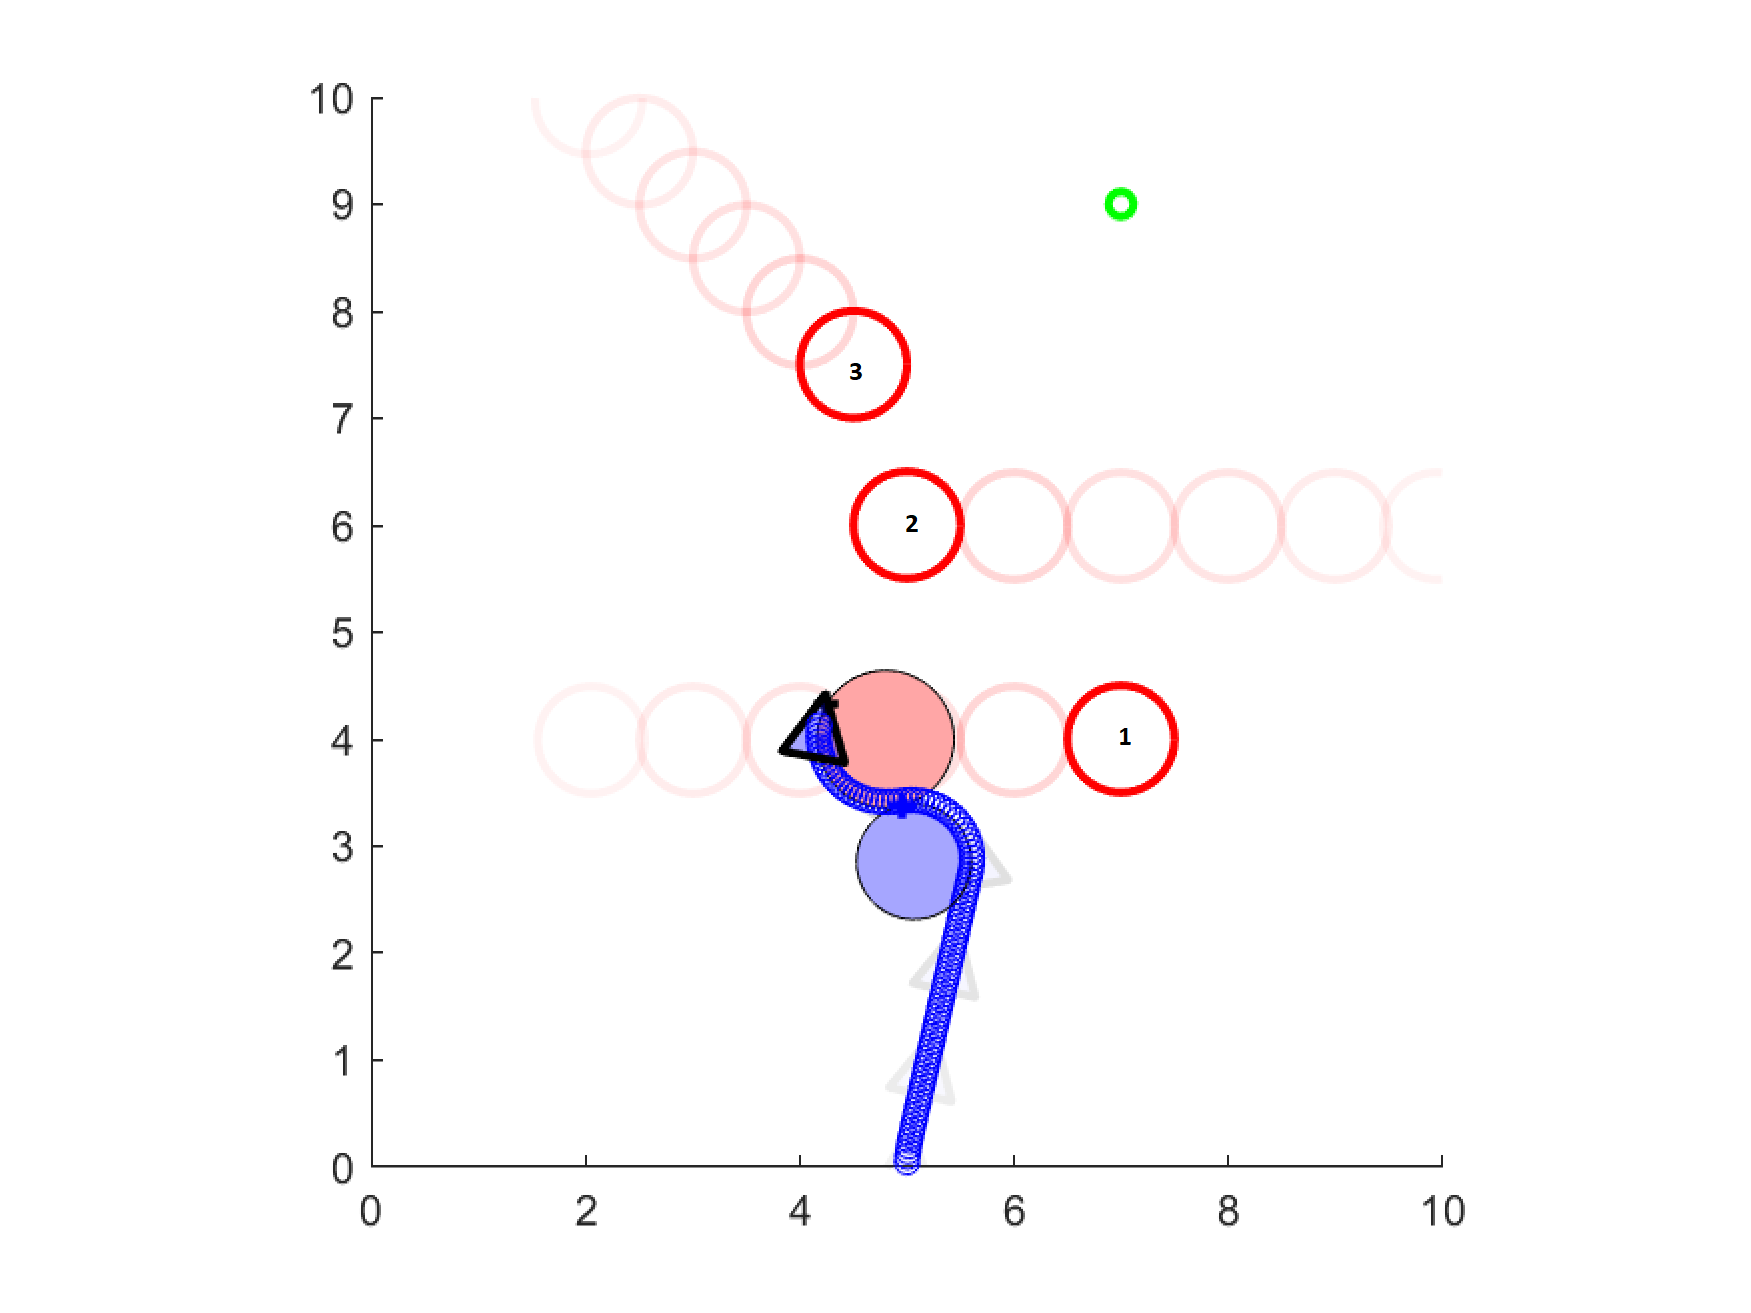
\includegraphics[width=\textwidth]{treobst_1.png}
\end{subfigure}
\hfill
\begin{subfigure}[t]{0.5\textwidth}
\centering
\caption{Bypassing del terzo ostacolo}
\label{bypass3}
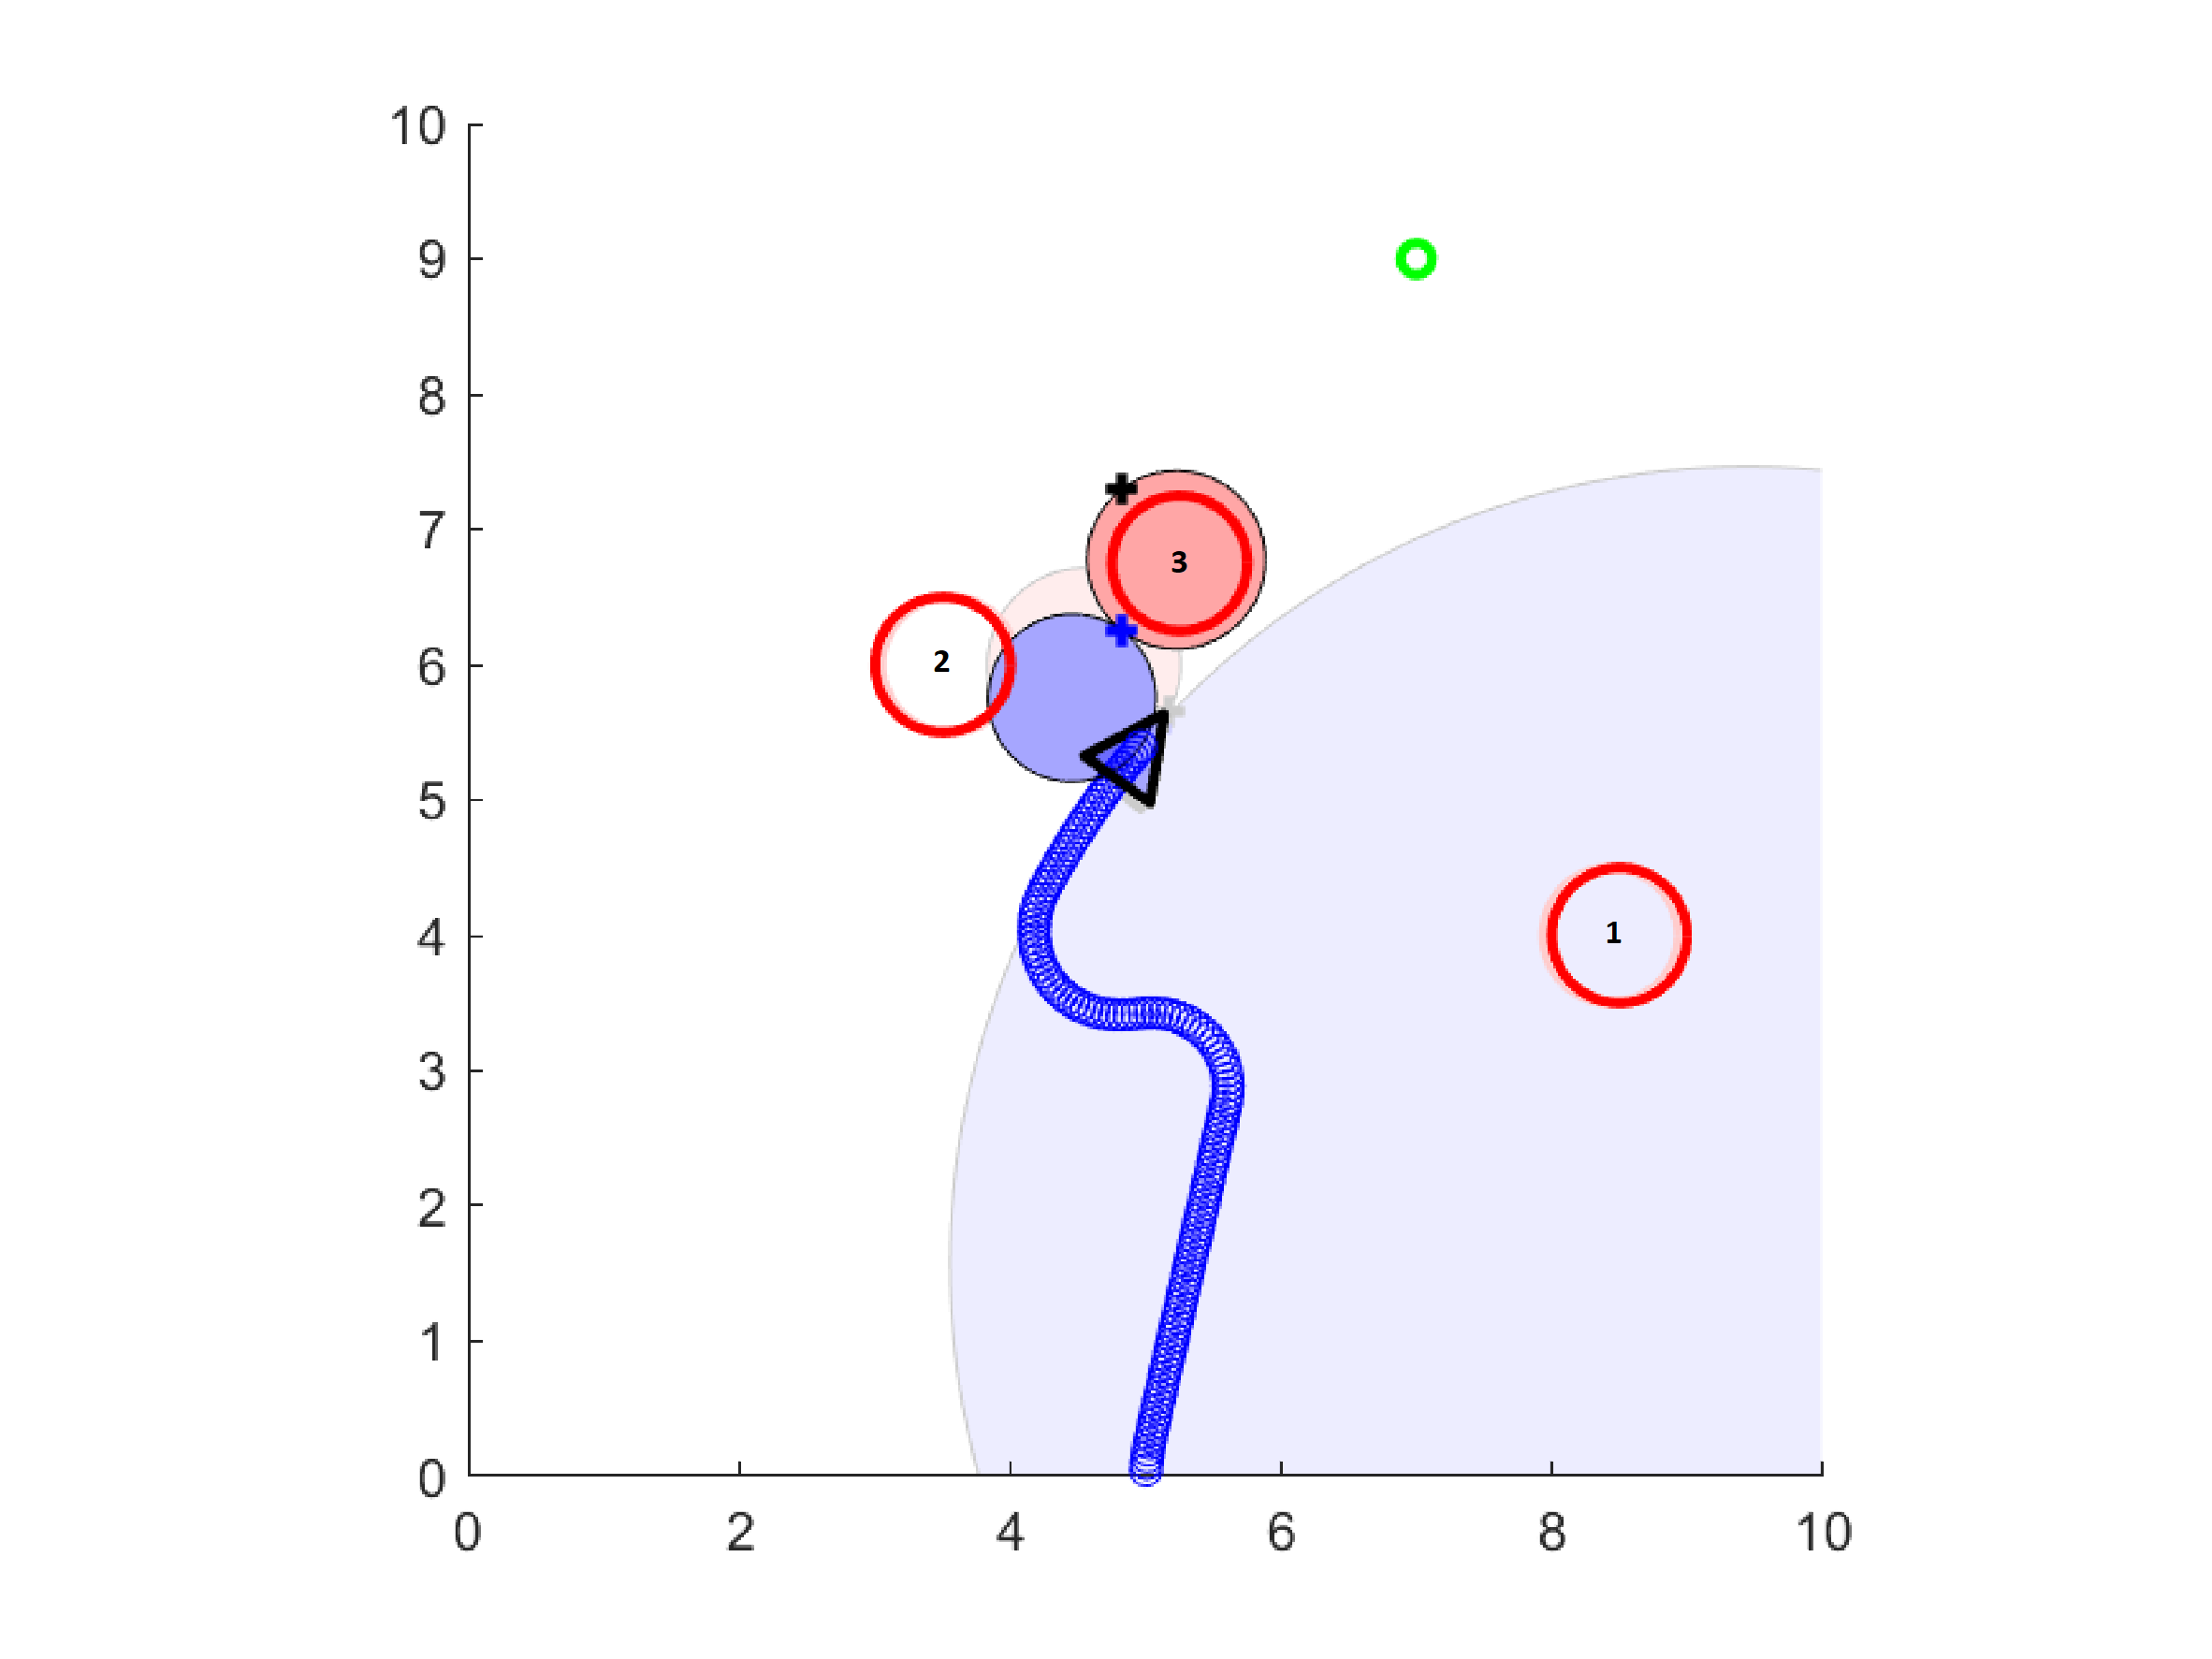
\includegraphics[width=\textwidth]{treobst_2.png}
\end{subfigure}
\caption{Snapshots della simulazione}
\label{snapshot1}
\end{figure}
In riferimento alla figura \ref{snapshot1}, i cerchi rossi vuoti indicano gli ostacoli in movimento. I cerchi rossi pieni indicano le circonferenze attorno all'ostacolo rilevato all'istante \(\tau\), mentre i cerchi blu pieni le circonferenze attorno all'ostacolo virtuale.\\
Alla fine, il robot avrà percorso la traiettoria riportata nel seguente snapshot. Il robot é arrivato con successo nel goal, evitando gli ostacoli incontrati.
\begin{figure}[H]
\centering
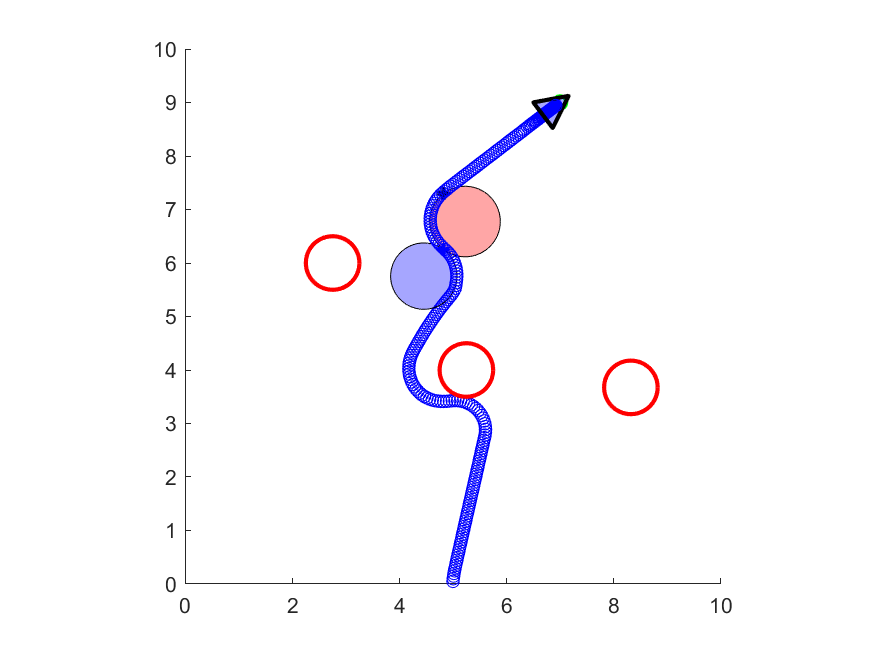
\includegraphics[width=0.8\textwidth]{treobst_finale.png}
\caption{Traiettoria finale}
\end{figure}

\subsection{Otto ostacoli fissi}
In figura \ref{moltiostacoli} si può notare come il robot gestisca, con una traiettoria continua e senza collidere con gli ostacoli, una situazione in cui, in proporzione alle dimensioni dell'ambiente (in questo caso 10x10[m]), risulti un'alta densità di ostacoli. In questo esempio sono stati ``immessi" nell'ambiente otto ostacoli fissi. Da notare che, visto che gli ostacoli sono fissi e il robot riceve questo informazione grazie al modulo di visione, lo spostamento dalla traiettoria ``principale" é minima, per mantenere l'ottimalità della traiettoria, ma sufficiente per non collidere con l'ostacolo.

\begin{figure}[H]
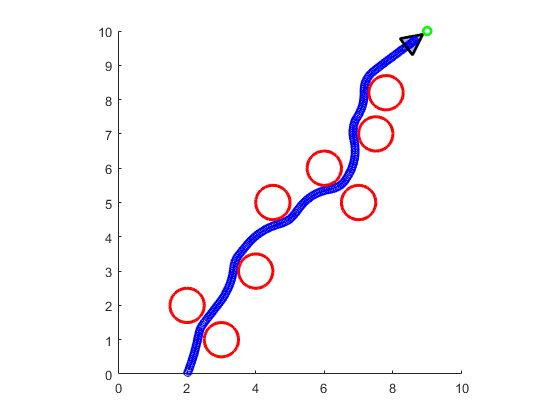
\includegraphics[width=\textwidth]{moltiostacoli.png}
\caption{Simulazione dell'algoritmo con otto ostacoli fissi}
\label{moltiostacoli}
\end{figure}

\subsection{Considerazione sul calcolo di h}

Un parametro sicuramente molto importante é il raggio h della circonferenza centrata nell'ostacolo da bypassare. Da esso dipende la capacità del robot di bypassare correttamente l'ostacolo, senza collidere durante il bypass.

\begin{figure}[H]
\begin{subfigure}[b]{0.5\textwidth}
\centering
\caption{Snapshot prima del bypass all'istante \(\tau\)}
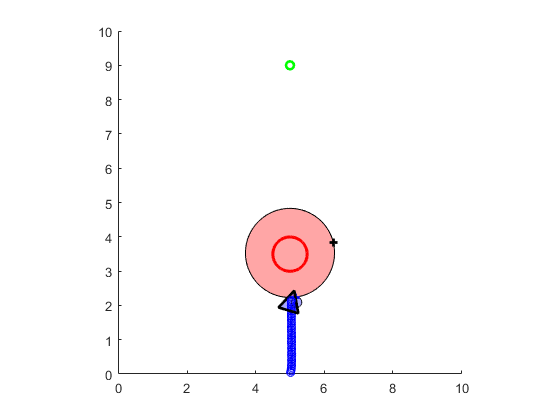
\includegraphics[width=\textwidth]{hmax_1.png}
\end{subfigure}
\hfill
\begin{subfigure}[b]{0.5\textwidth}
\centering
\caption{Snapshot durante il bypass}
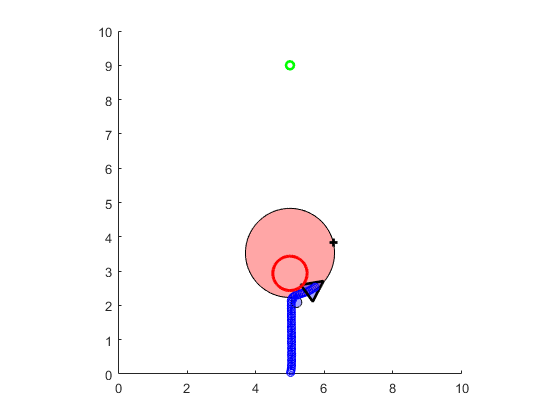
\includegraphics[width=\textwidth]{hmax_2.png}
\end{subfigure}
\vfill
\begin{subfigure}[b]{0.5\textwidth}
\centering
\caption{Snapshot all'istante \(\tau+\Delta t_{bypass}\)}
\label{hmax2}
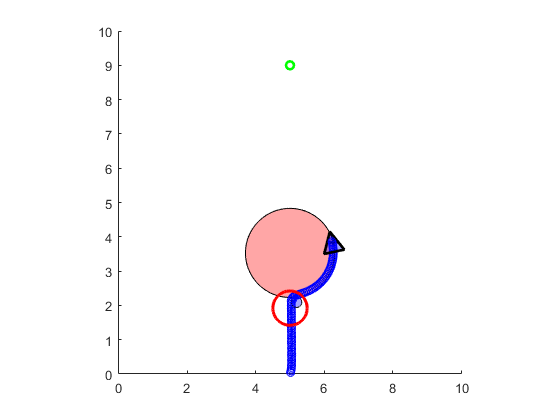
\includegraphics[width=\textwidth]{hmax_3.png}
\end{subfigure}
\hfill
\begin{subfigure}[b]{0.5\textwidth}
\centering
\caption{Snapshot nella posizione finale}
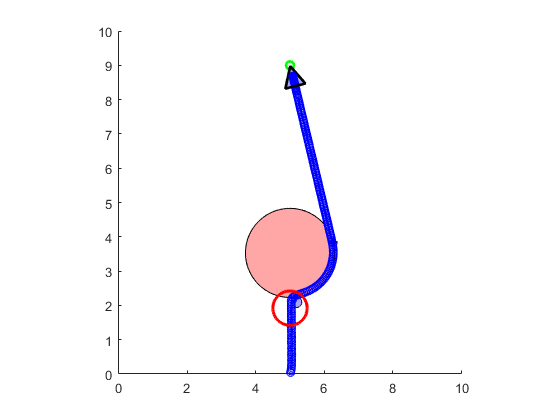
\includegraphics[width=\textwidth]{hmax_4.png}
\end{subfigure}
\caption{Bypassing con grado di invasività massimo}
\label{hmax}
\end{figure}
\begin{nota}
Da notare che il cerchio rosso vuoto indica l'ostacolo, mentre quello pieno indica la circonferenza attorno all'ostacolo all'istante \(tau\). In figura \ref{hmax2} l'ostacolo (cerchio rosso vuoto) si trova, all'istante \(t=\tau+\Delta t_{bypass}\) - dove \(\Delta t_{bypass}\) é una durata legata al bypass - in posizione \([5,2]\), ovvero lì dove si trovava il robot all'istante \(t=\tau\). Perciò non vi é nessuna collisione, visto che a \(t=\tau+\Delta t_{bypass}\) il robot si trova, ispezionando la figura, in posizione circa \([6,4]\).
\end{nota}
In figura \ref{hmax} si nota come il robot bypassi l'ostacolo tenendosi ad una distanza di sicurezza piuttosto elevata. Ciò é dovuto al fatto che il grado di invasività é massimo, per cui il robot deve spostarsi dalla sua traiettoria più in fretta possibile. Con un h più piccolo ci sarebbe stata quasi sicuramente una collisione, mentre con h più grande il robot avrebbe dovuto tenersi ad una distanza di sicurezza pari praticamente al raggio di visione, il che avrebbe comportato una curvatura troppo brusca (si nota che già in queste condizioni la curvatura non é molto ``gentile").\\
In figura \ref{hmin} (per semplicità si riporterà soltanto gli snapshot durante e dopo il bypassing) invece, si può assistere ad un caso in cui il grado di invasività dell'ostacolo é minimo. Il robot, nei confronti del caso precedente si sposta molto meno dalla sua traiettoria e il tempo impiegato per bypassare é anche minore.

\begin{figure}[H]
\begin{subfigure}[t]{0.5\textwidth}
\centering
\caption{Durante il bypassing}
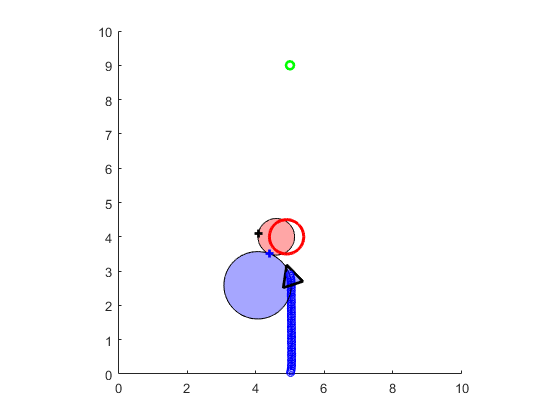
\includegraphics[width=\textwidth]{hmin_1.png}
\end{subfigure}
\hfill
\begin{subfigure}[t]{0.5\textwidth}
\centering
\caption{Dopo il bypassing}
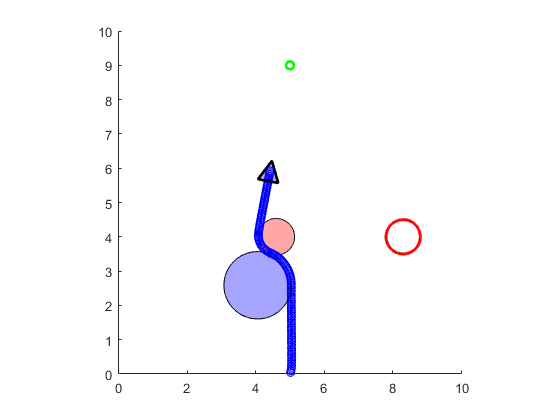
\includegraphics[width=\textwidth]{hmin_2.png}
\end{subfigure}
\caption{Bypassing con grado di invasività minimo}
\label{hmin}
\end{figure}


\subsection{Considerazione sullo switch al potenziale attrattivo}

Collegandosi alla sezione precedente, un'ulteriore considerazione che si potrebbe fare riguarda la durata dello switch: può succedere che, a fronte di una durata piuttosto breve in cui il robot potrebbe collidere con l'ostacolo, la traiettoria fa un giro più largo, allungando così il tempo rispetto a quello effettivamente necessario per eliminare l'ostacolo dal raggio di visione. Dalla figura \ref{nongiraprima} si può intuire che l'ostacolo aveva già percorso parecchi metri quando il robot stava ancora finendo di bypassare. Naturalmente, questo prolungamento temporale é giustificato dalla necessità di rendere la traiettoria continua durante gli switch.\\
Si potrebbe, tuttavia, scegliere di variare l'algoritmo e fare in modo che il robot passi al potenziale attrattivo non appena l'ostacolo da bypassare non é più nel suo raggio di visione (e nel tubo direzionato). Ne consegue che la traiettoria é quella mostrata in figura \ref{giraprima}, in cui vediamo una curvatura più ripida in corrispondenza dello switch dal potenziale bypassante a quello attrattivo. Si può notare, però, che, a parità di tempo trascorso (i due ostacoli si trovano nella stessa posizione nello snapshot) il robot nel secondo caso é più vicino al goal. Dunque, a fronte di un tempo minore per arrivare nel goal, bisogna sacrificare la continuità della traiettoria. 

\begin{figure}[H]
\begin{subfigure}[t]{0.5\textwidth}
\centering
\caption{Il robot switcha in P2}
\label{nongiraprima}
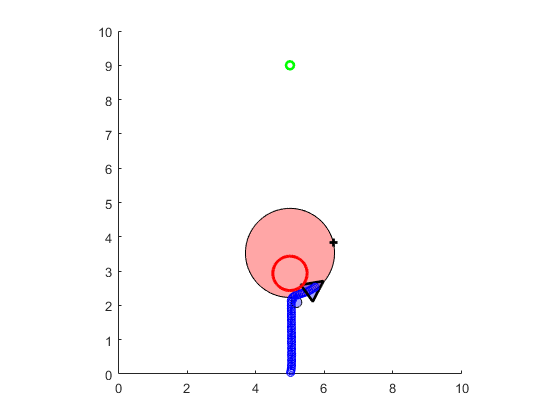
\includegraphics[width=\textwidth]{hmax_2.png}
\end{subfigure}
\hfill
\begin{subfigure}[t]{0.5\textwidth}
\centering
\caption{Il robot switcha prima}
\label{giraprima}
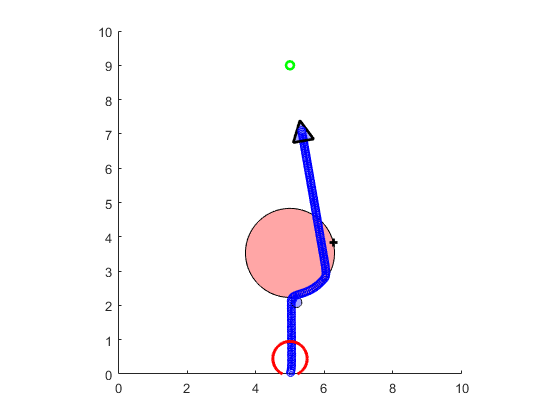
\includegraphics[width=\textwidth]{giraprima.png}
\end{subfigure}
\caption{Alternativa allo switching in P2}
\label{snapshot1}
\end{figure}

\subsection{Minimi locali}
Come ultimo esempio si considera un caso in cui nel metodo classico é limitante il problema dei minimi locali. A tal fine la configurazione di partenza é \(G = [6,10]\), \(O_1=[5,4]\) con \(v_1=[0,0]\) e \(O_2=[7,4]\) con \(v_2=[0,0]\) (entrambi gli ostacoli sono fermi). Il moto del robot inizia da \([5,0]\). In figura \ref{minimolocalesim} si può vedere che il robot (gli scatter points rossi) compie un percorso che inizialmente va verso il goal (il minimo), ma, una volta arrivato vicino ai due ostacoli, inizia a ruotare sullo stesso punto. Ciò é dovuto al fatto che non vi é nessuna forza a spingerlo avanti, conseguentemente al fatto che i potenziali repulsivi e attrattivi si annullano a vicenda in quel punto.
\begin{figure}[H]
\centering
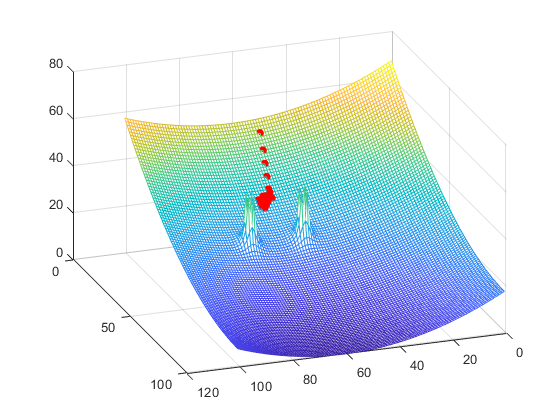
\includegraphics[width=0.7\textwidth]{minimolocalesim.png}
\caption{Path planning con metodo classico}
\label{minimolocalesim}
\end{figure}
Al contrario, con l'algoritmo sviluppato in questo lavoro di tesi, il problema dei minimi locali é assente. Il robot rileva l'ostacolo alla sinistra, lo evita e non si fa ``disturbare" dall'ostacolo alla destra, che non intralcia minimamente l'avanzamento verso il goal.  
\begin{figure}[H]
\centering
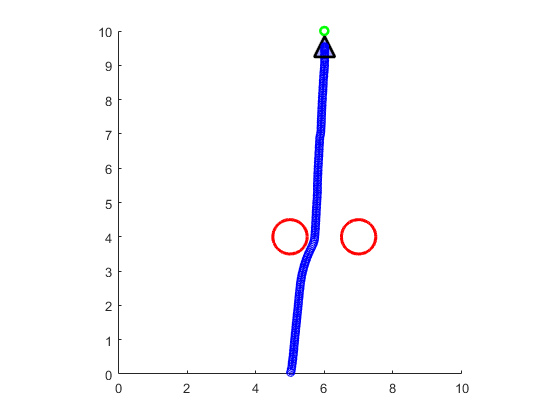
\includegraphics[width=0.8\textwidth]{nominimolocalesim.png}
\caption{Path planning con metodo bypassante}
\label{minimolocalesim}
\end{figure}
Ciò é un esempio lampante del concetto ``all'algoritmo non servono informazioni globali riguardanti gli altri ostacoli": se nel metodo classico, infatti, il moto del robot viene influenzato non solo dall'ostacolo più vicino (da aggirare), ma anche da quelli più lontani, nel metodo proposto nel presente elaborato il robot fa esclusivamente uso di ciò che succede nel suo raggio di visione, agendo di conseguenza. Quindi, come ribadito anche nel paragrafo precedente, la scelta del raggio di visione (e anche della distanza di sicurezza dagli ostacoli) é cruciale per una buona riuscita del path planning. Un raggio di visione troppo grande potrebbe risultare in un ``overkill", nel senso che il robot potrebbe voler evitare ostacoli che in realtà sono molto lontani; un raggio di visione troppo piccolo sfocerebbe eventualmente in una collisione.
\newpage
\section{Conclusione}
Le applicazioni dell'algoritmo di path planning sono ovviamente innumerevoli, come lo sono anche le espansioni future.\\
Come già detto precedentemente, l'algoritmo può essere facilmente integrato con un modulo di visione ad-hoc. Allo stesso modo, può essere adattato ad ambienti specifici, ad esempio mappe di ambienti chiusi, e integrato con tecniche di SLAM \cite{slam}. Brevemente, queste tecniche consistono nel localizzare il robot localmente e costruire la mappa mentre esso esplora l'ambiente. \\
Casi studio interessanti possono essere anche quelli in cui gli ostacoli siano di forma diversa e non circolari, come supposto in questo lavoro di tesi. Un'altra generalizzazione che si può fare in merito agli ostacoli riguarda il loro movimento: può essere studiato un movimento a ``zig-zag" e possono essere analizzate possibili situazioni di stallo.\\
Un'ulteriore espansione che si potrebbe fare sarebbe rendere l'algoritmo di path planning distribuito, ovvero ideale per un sistema multi-agente che sia coordinato per raggiungere un obiettivo comune, come ad esempio nel robot soccer.\\
In conclusione, in questo lavoro di tesi si é implementato un algoritmo di path planning locale per robot mobili basato su un meccanismo di switching tra potenziali artificiali, sfruttando un diverso tipo di potenziale (bypassante). Si assicura con l'algoritmo implementato che il robot possa sempre giungere in una posa dalla quale é capace di raggiungere il goal e di evitare gli ostacoli (fissi o in movimento). Il metodo é stato testato numericamente in ambiente Matlab e si é rivelato efficace, anche con più ostacoli in movimento.

\newpage \lstlistoflistings
\newpage \listoffigures \printbibliography

\end{document}
